%% Compile me as follows:
%%% latexmk -pdf -xelatex -shell-escape presentation.tex

\documentclass[xetex,compress]{beamer}
%% \usetheme{Pittsburgh}
%% \usecolortheme{seagull}

%% https://www.quora.com/Presentations-What-are-the-best-beamer-themes
\setbeamertemplate{frametitle}
  {\begin{centering}\smallskip
   \insertframetitle\par
   \smallskip\end{centering}}
\setbeamertemplate{itemize item}{\(\bullet\)}
\setbeamertemplate{navigation symbols}{}
\setbeamertemplate{footline}[text line]{%
    \hfill\strut{%
        \scriptsize\sf\color{black!60}%
        \quad\insertframenumber
    }%
    \hfill
}
%% \setbeamertemplate{caption}{\raggedright\insertcaption\par}

% Define some colors:
\definecolor{PittBlue}{RGB}{0,43,94}
\definecolor{PittGold}{RGB}{197,168,118}
\definecolor{DarkFern}{HTML}{407428}
\definecolor{DarkCharcoal}{HTML}{4D4944}
\colorlet{Fern}{DarkFern!85!white}
\colorlet{Charcoal}{DarkCharcoal!85!white}
\colorlet{LightCharcoal}{Charcoal!50!white}
\colorlet{AlertColor}{orange!80!black}
\colorlet{DarkRed}{red!70!black}
\colorlet{DarkBlue}{blue!70!black}
\colorlet{DarkGreen}{green!70!black}
% Use the colors:
\setbeamercolor{title}{fg=PittBlue}
\setbeamercolor{frametitle}{fg=PittBlue}
\setbeamercolor{normal text}{fg=DarkCharcoal}
\setbeamercolor{block title}{fg=black,bg=Fern!25!white}
\setbeamercolor{block body}{fg=black,bg=Fern!25!white}
\setbeamercolor{alerted text}{fg=AlertColor}
\setbeamercolor{itemize item}{fg=Charcoal}

\usepackage[utf8]{inputenc}
\usepackage[T1]{fontenc}
\usepackage{alltt}
\usepackage{bm}
\usepackage[normalem]{ulem}
\usepackage{paralist}
\usepackage{setspace}
\usepackage{xparse}
\usepackage{braket}
\usepackage{wrapfig}
\usepackage[export]{adjustbox}
\usepackage{booktabs}

\makeatletter
\g@addto@macro\@floatboxreset\centering
\makeatother

\DeclareDocumentCommand{\vect}{m}{
        \ensuremath{\boldsymbol{\mathbf{#1}}}
}

%%% Chemistry
\usepackage{chemformula}

\makeatletter
\newcommand\listofframes{\@starttoc{lbf}}
\makeatother

\addtobeamertemplate{frametitle}{}{%
  \addcontentsline{lbf}{section}{\protect\makebox[2em][l]{%
    \protect\usebeamercolor[fg]{structure}\insertframenumber\hfill}%
  \insertframetitle\par}%
}

\setbeamertemplate{navigation symbols}{}

%%%%%%%%%%%%%%%%%%%%%%%%%%%%%%%%%%%%%%%%%%%%%%%%%%%%%%%%%%%%%%%%%%%%%%%%%%%%%%

\title{Deciphering the Contents of Chemically-Trained Neural Networks into Physical Intuition}
\author[Berquist]{Eric Berquist}
%% \institute[Pitt]{University of Pittsburgh}
\institute[Pitt]{
\includegraphics[width=1in]{./figures/pitt_logo.pdf}}
\date{June 15th, 2017}

\begin{document}

\frame{
  \titlepage
}

\begin{frame}{Overview}
  Machine learning (ML) is seeing rapid growth in areas relevant to quantum chemistry, but how does it work?
  \begin{itemize}
  \item \underline{Topic}: Are correct ML predictions in quantum chemistry \emph{right for the right reasons}?
  \item \underline{Gap}: We don't know if current approaches (ML architectures) will work more complex molecules or properties.
  \item \underline{Rationale}: If a ML model is not right for the right reasons, there cannot be an expectation that it is transferable or extendable in any way.
  \end{itemize}
  We need to know if ML models are learning chemistry and not just numbers (von Neumann's elephant).
\end{frame}

\begin{frame}{Overview}
  \begin{itemize}
  \item The \underline{objective} is to quantify what ML models trained on quantum chemical data are learning.
  \item The \underline{central hypothesis} is that models are learning about molecular structure identically to how we apply chemical intuition.
  \end{itemize}
  This hypothesis will be tested by
  \begin{itemize}
  \item training neural networks (NNs) to replicate literature results,
  \item ``seeing'' what the currently-available models have learned using \textbf{relevance propagation},
  \item attempt to predict more complex molecular properties than those found in the literature, and
  \item quantify if learning changes for more complex properties.
  \end{itemize}
\end{frame}

\begin{frame}{\protect\alert{!!! Disclaimer !!!}}
  The goal of this work is \emph{not} to produce more accurate or more transferable models. The goal is to understand \emph{how} and \emph{why} models make (in)accurate predictions in terms of what they have learned.
\end{frame}

\begin{frame}{What is machine learning?}
  Arthur Samuel (IBM), 1959: the subfield of computer science that gives
  \begin{quote}
    computers the ability to learn without being explicitly programmed.
  \end{quote}
  Tom Mitchell (CMU), 1997:
  \begin{quote}
    A computer program is said to learn from experience \textit{E} with respect to some class of tasks \textit{T} and performance measure \textit{P} if its performance at tasks in \textit{T}, as measured by \textit{P}, improves with experience \textit{E}.
  \end{quote}
\end{frame}

\begin{frame}{Machine learning will solve all our problems}
  \begin{center}
    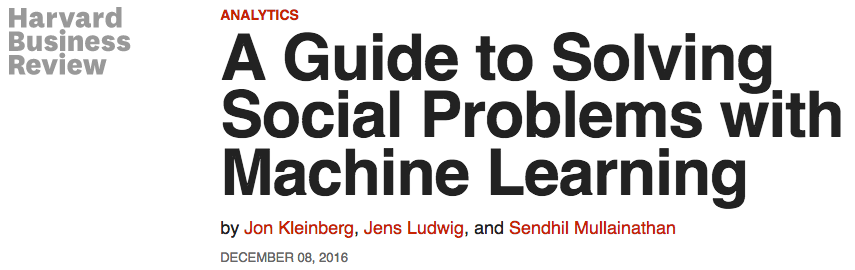
\includegraphics[width=1.00\textwidth]{./figures/headline.png}
  \end{center}
\end{frame}

\begin{frame}{Machine learning will solve all our problems}
  \begin{center}
    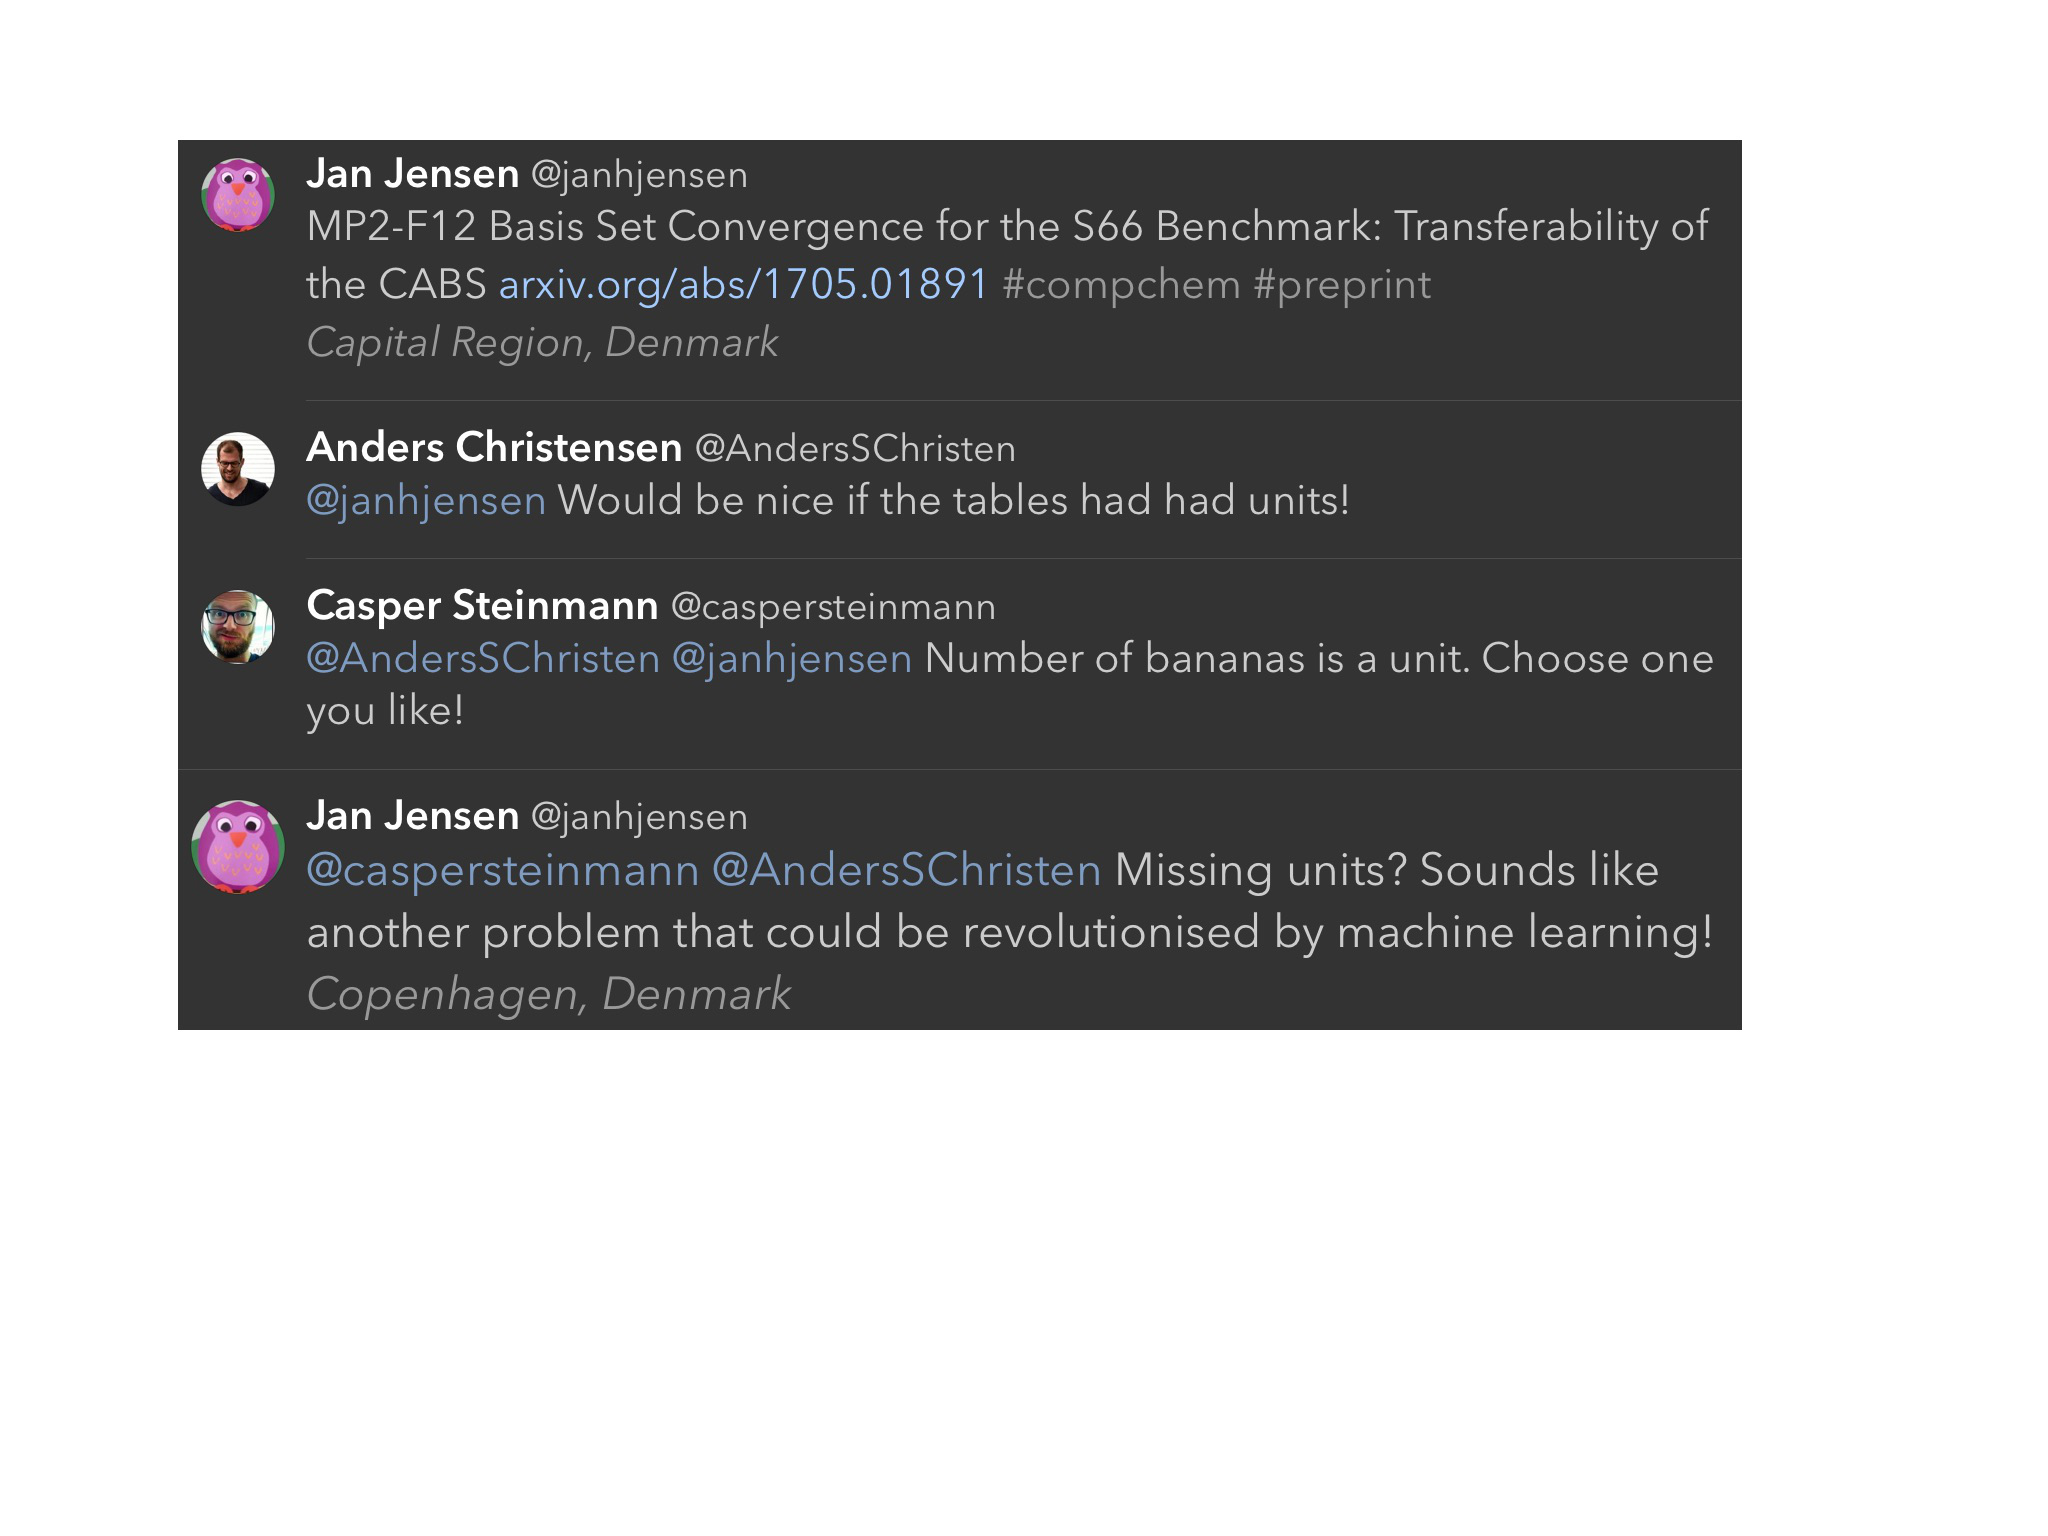
\includegraphics[width=1.10\textwidth]{./figures/twitter.jpeg}
  \end{center}
\end{frame}

\begin{frame}{}
  \begin{center}
    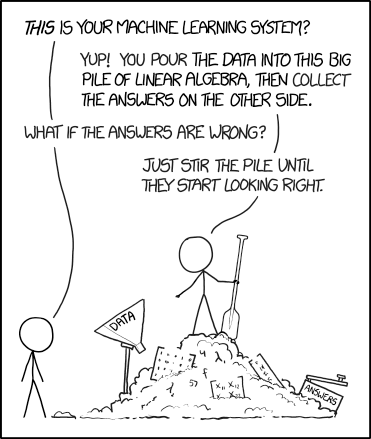
\includegraphics[width=0.75\textwidth]{./figures/machine_learning.png}
  \end{center}
\end{frame}

\begin{frame}{Machine learning has a perception problem}
  Machine learning is a ``fad'' and produces all these great results, but we joke semi-seriously that we don't know what's going on under the hood, even though it will solve all our problems.
  \begin{center}
    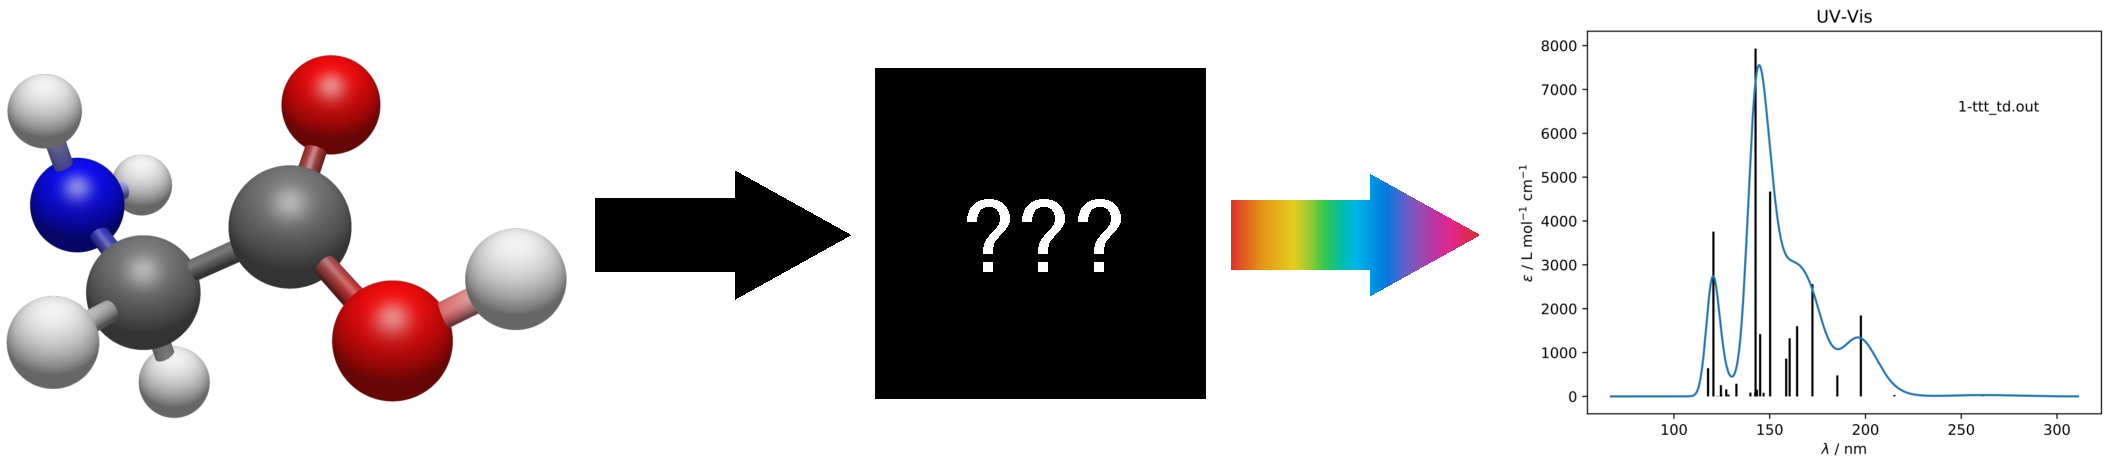
\includegraphics[width=1.00\textwidth]{./figures/black_box_prediction.pdf}
  \end{center}
\end{frame}

\begin{frame}{Objective}
  \begin{itemize}
  \item Peek inside the black box and see if ML models are ``learning chemistry''.
  \item If they aren't, consider other NN architectures (DTNN, ANAKIN-ME, ...) that have different input \textit{representations} or \textit{featurizations} for molecules, or
  \item make the architecture larger and use more training data.
  \end{itemize}
\end{frame}

\begin{frame}{Rationale}
  \begin{itemize}
  \item Building complex ML models that can do real, useful chemistry in a \emph{general} manner is impossible without proving meaningfulness of simpler models.
  \item Clearly the dozen or so papers from 2016-2017 show that accurate predictions can be made even under the assumption of black-box models.
  \item Additionally, if we can interpret the model directly, then perhaps eventually we can interpret chemistry using the model itself and not just predictions.
  \end{itemize}
\end{frame}

\begin{frame}{Rationale}
  Is it alright to accept the use of NNs that are not truly transferable (B3LYP, M06)? Maybe this works for prediction results, but we will repeat the history of DFT.
  \begin{center}
    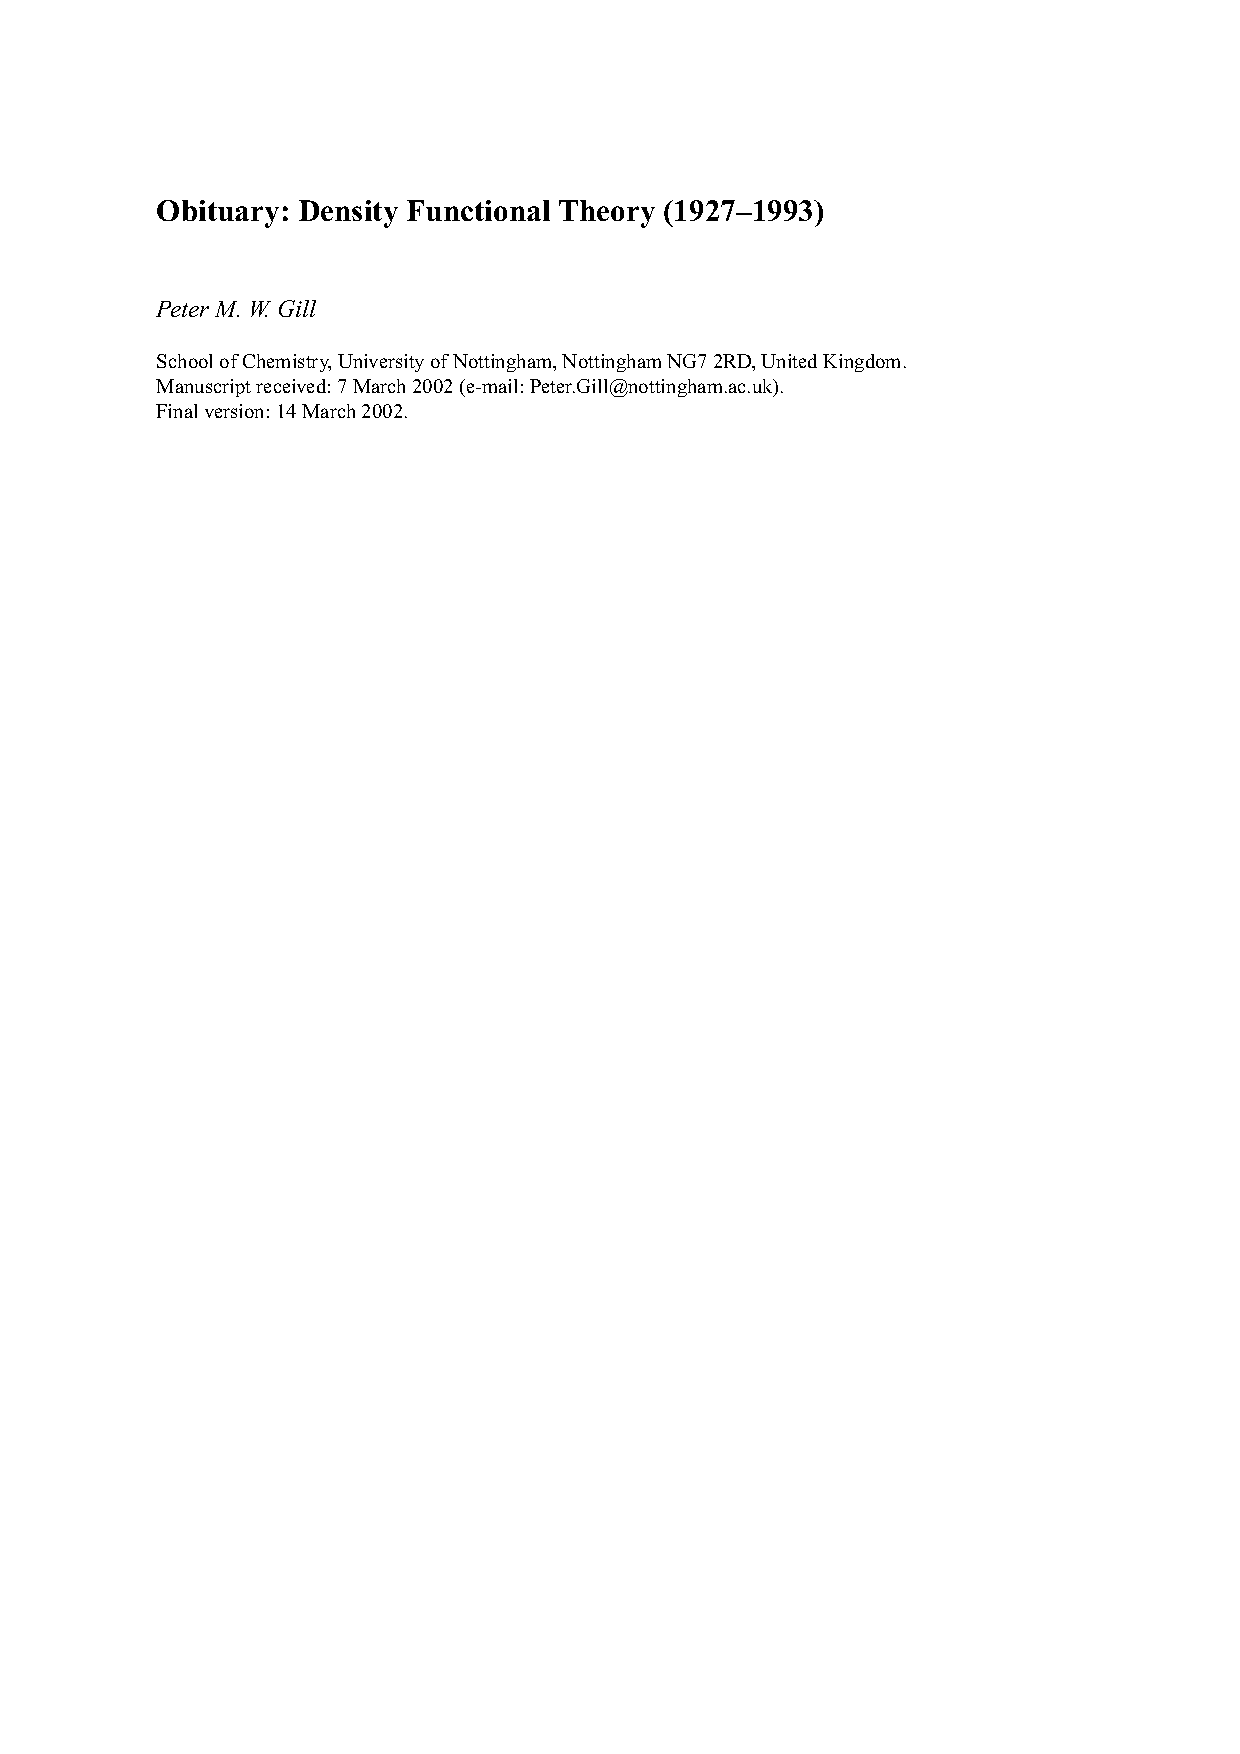
\includegraphics[width=1.00\textwidth]{./figures/obit.pdf}
  \end{center}
\end{frame}

\begin{frame}{}
  \begin{center}
    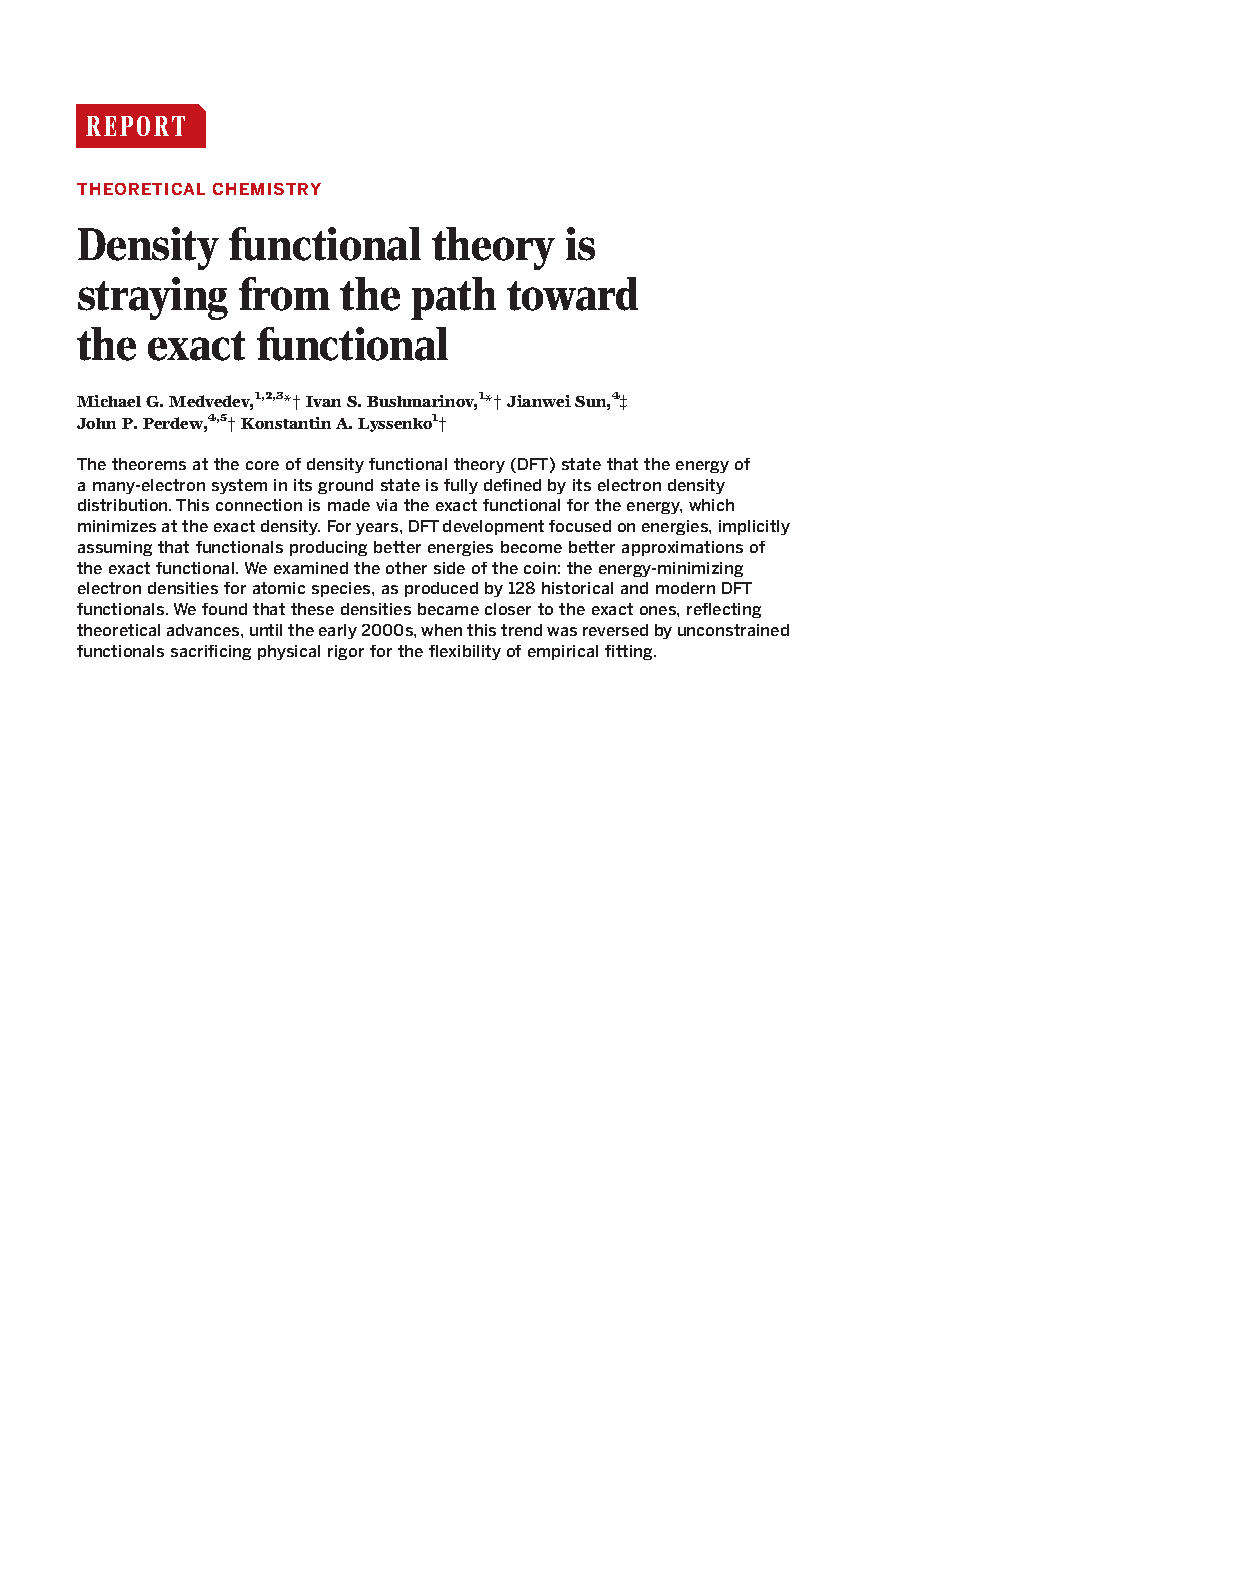
\includegraphics[width=1.00\textwidth]{./figures/obit2.pdf}
  \end{center}
\end{frame}

\begin{frame}{Transferability}
  Literature usage:
  \begin{itemize}
  \item No need for reparametrization from system to system
  %% \item More to do with the \underline{input representation} than the \underline{molecules} it can be applied to
  \item Limited to organic molecules, train small (9 heavy atoms), test larger (10 heavy atoms)
  \item Charge and spin: neutral and closed-shell singlet
  \end{itemize}
  A better definition in terms of examples:
  \begin{itemize}
  \item Does the same model work for optimized and non-equilibrium (MD) structures?
  \item Does the model work for charged systems?
  \item Does the model work for systems with unpaired electrons?
  \end{itemize}
\end{frame}

\begin{frame}{Specific Aims}
  \begin{itemize}
  %% \item[1.] Reproduction of Existing Literature Neural Networks
  %% \item[2.] Characterization of Existing Literature Neural Networks
  %% \item[3.] Training Neural Networks for Complex Molecular Properties
  %% \item[4.] Characterization of Novel Neural Networks
  \item[1.] Reproduce existing neural network models for molecular properties from the literature.
  \item[2.] Characterize the parameters learned by existing neural network models from the literature using relevance propagation.
  \item[3.] Train supervised neural networks on complex molecular properties.
  \item[4.] Characterize the parameters learned for complex molecular properties using relevance propagation and unsupervised neural networks.
  \end{itemize}
\end{frame}

%% \begin{frame}{Background}
%%   \begin{itemize}
%%   \item Introduction to machine learning
%%   \item Simplest form: univariate linear regression
%%   \item Neural networks (NNs)
%%   \item Linear regression using a NN
%%   \item More complex neural networks
%%   \item Training neural networks
%%   \item Relevance propagation: examples
%%   \item Relevance propagation: analogies go here
%%   \end{itemize}
%% \end{frame}

\begin{frame}{Background}
\end{frame}

\begin{frame}{Introduction to machine learning}
  \textbf{Supervised learning}:
  \begin{itemize}
  \item Learn to predict an output given an input
  \end{itemize}
  \textbf{Unsupervised learning}:
  \begin{itemize}
  \item Discover a good internal representation of the input
  \item Learn to reconstruct the input from itself \emph{non-trivially}
  \end{itemize}
\end{frame}

\begin{frame}{Introduction to machine learning}
  \textbf{Classification}:
  \begin{itemize}
  \item Given a set of data, identify the classes that the data belongs to
  \item Predict what group a piece of data is a member of
  \item Output: Discrete, categorical
  \item Example: \(x\) could be a cat, dog, or bird, and is a bird \(\rightarrow y = (0, 0, 1)\)
  \end{itemize}
  \textbf{Regression}:
  \begin{itemize}
  \item Given a set of data, find the best relationship that represents the set of data
  \item Output: Continuous, numerical
  \item Example: Find \(m\) and \(b\) in \(y=mx+b\)
  \end{itemize}
\end{frame}

\begin{frame}{Simplest form: univariate linear regression}
  \underline{Hypothesis}:
  \begin{equation*}
    h_{\theta}(x) = \theta_0 + \theta_1 x
  \end{equation*}
  \underline{Parameters}:
  \begin{equation*}
    \theta_{0}, \theta_{1}
  \end{equation*}
  \underline{Cost/penalty function} (\(m = \text{\# of training inputs}, y = \text{exact prediction}\)):
  \begin{equation*}
    J(\theta_{0}, \theta_{1}) = \frac{1}{2m} \sum_{i=1}^{m} \left( h_{\theta}(x^{(i)}) - y^{(i)} \right)^2
  \end{equation*}
  \underline{Goal}:
  %% https://tex.stackexchange.com/questions/73226/how-to-write-something-underneath-min#73228
  \begin{equation*}
    \min_{\theta_{0}, \theta_{1}} J(\theta_{0}, \theta_{1})
  \end{equation*}
\end{frame}

\begin{frame}{Parameter optimization}
  Finding the set of coefficients that minimize the cost function:
  %% https://tex.stackexchange.com/questions/6195/typeset-an-with-an-above#6196
  \begin{align*}
    \frac{\partial J}{\partial \theta_{j}} &\overset{!}{=} 0 \\
    &= \frac{1}{m} \sum_{i=1}^{m} \left( h_{\theta}(x^{(i)}) - y^{(i)} \right) x^{(i)}
  \end{align*}
  which are used in gradient descent (or an equivalent) algorithm:
  \begin{align*}
    \text{repeat until convergence \{} \\
    \theta_{j} := \theta_{j} - \eta \frac{\partial}{\partial \theta_{j}} J(\theta_{0},\theta_{1}) \\
    (\text{for }j = 1\text{ and }j = 0) \\
    \text{\}}
  \end{align*}
  \(\eta\) is the learning rate (a \underline{hyperparameter}).
\end{frame}

\begin{frame}{Linear regression using a neural network}
  \begin{center}
    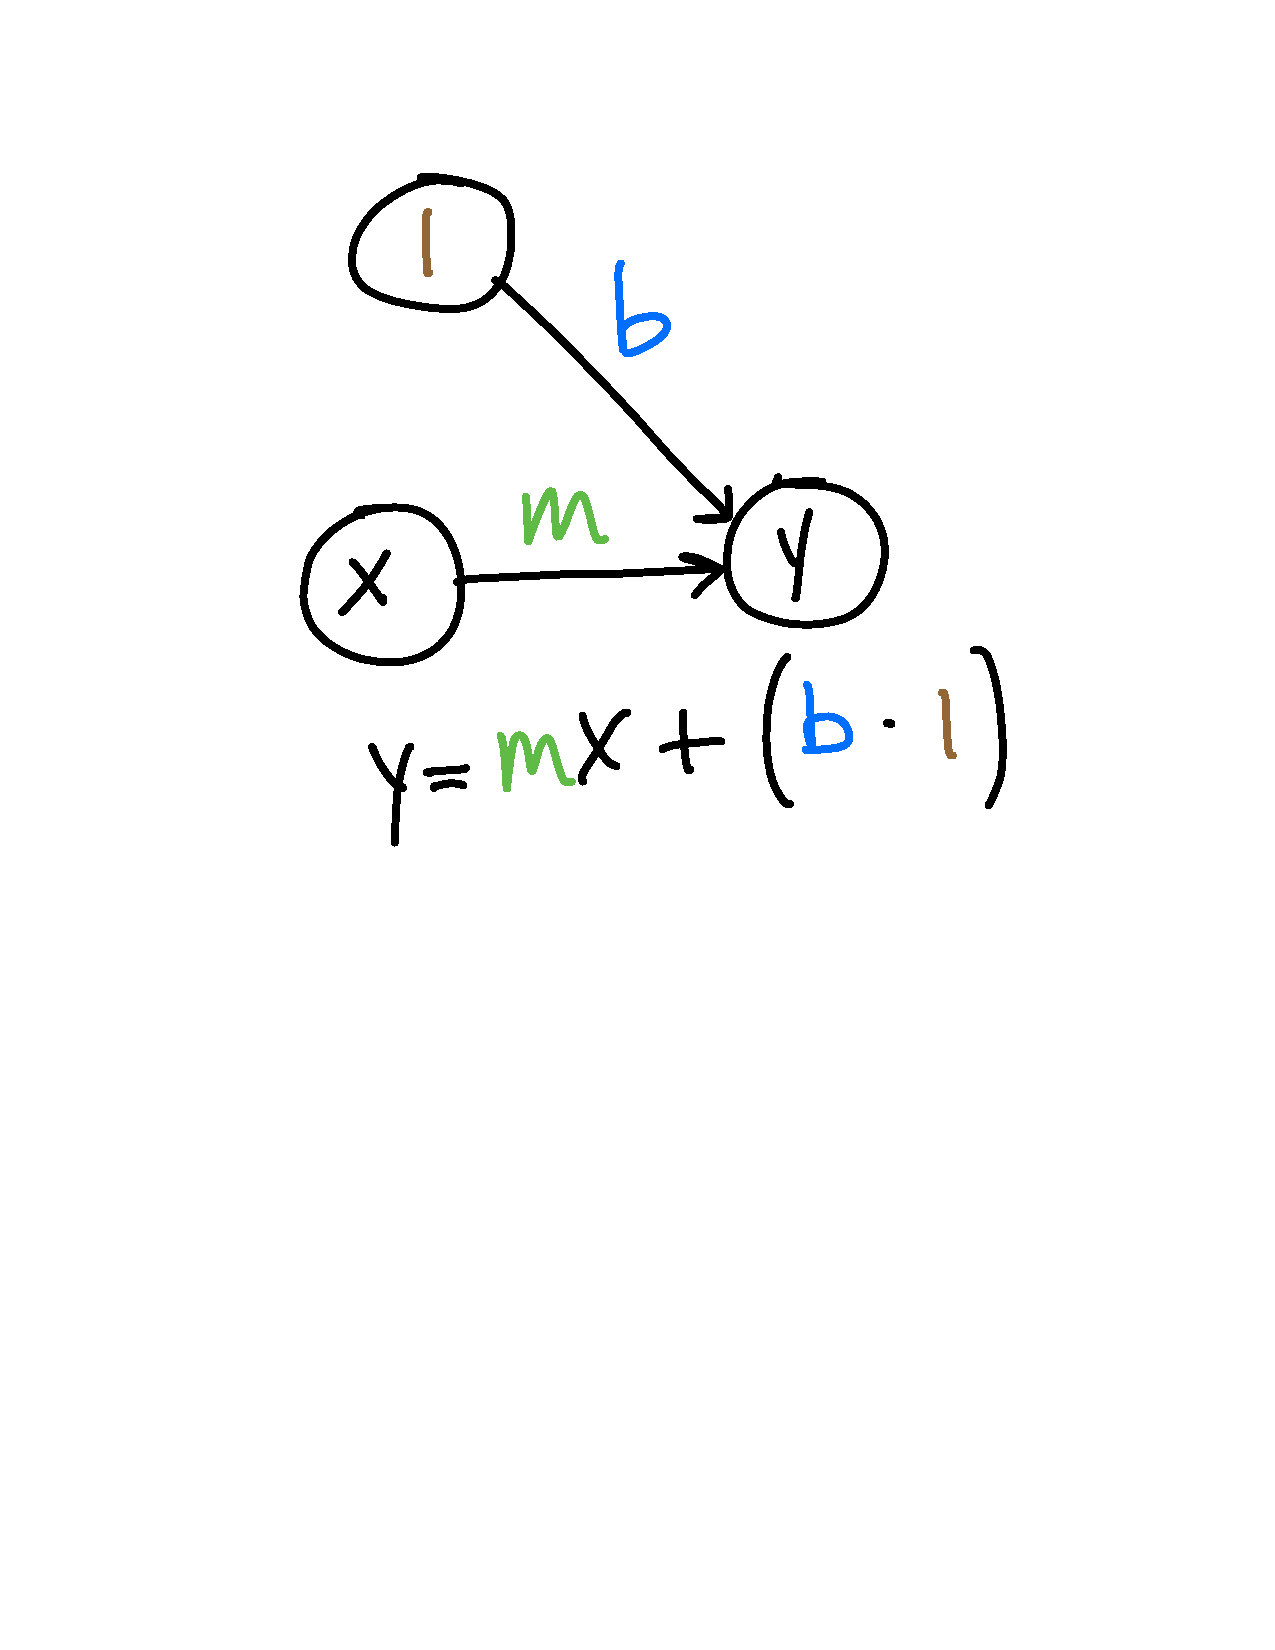
\includegraphics[width=0.75\textwidth]{./figures/lr_nn_1.pdf}
  \end{center}
\end{frame}

\begin{frame}{Linear regression using a neural network}
  \begin{center}
    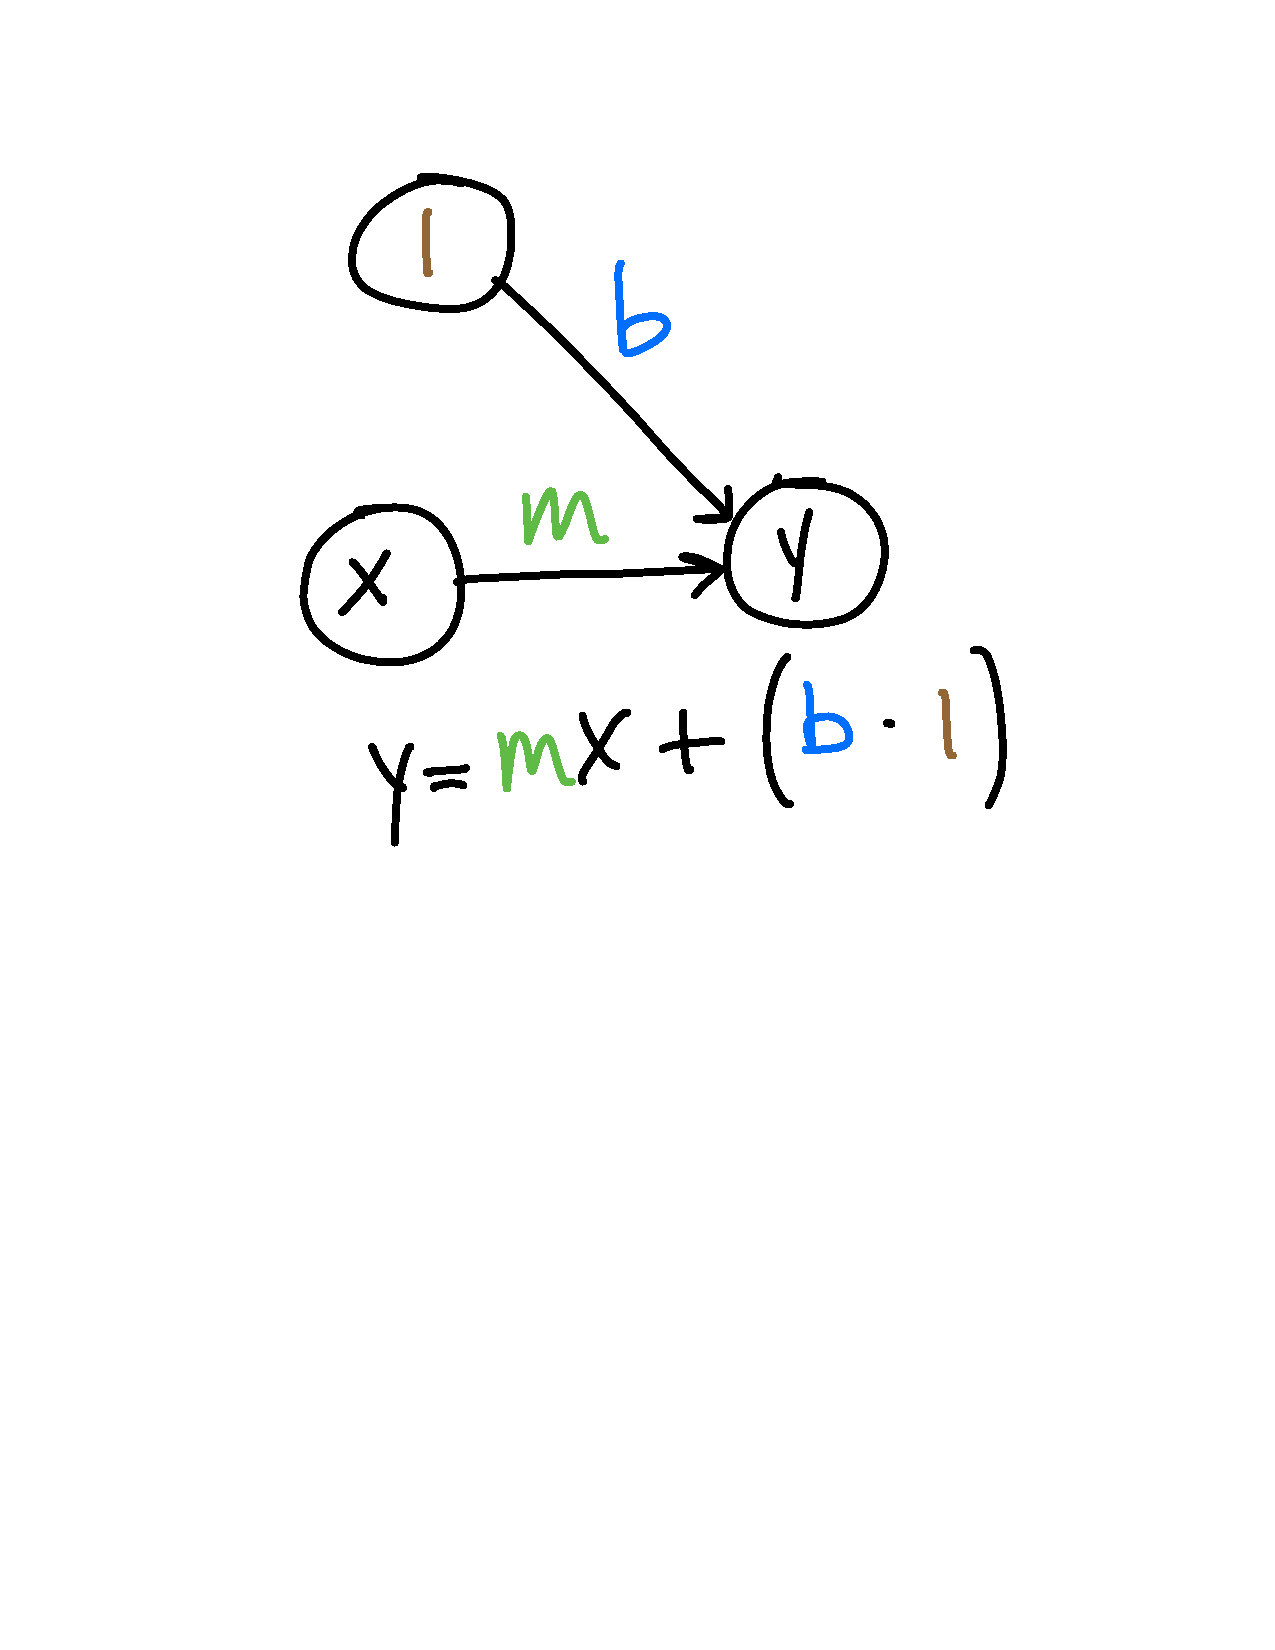
\includegraphics[width=0.50\textwidth]{./figures/lr_nn_1.pdf}
    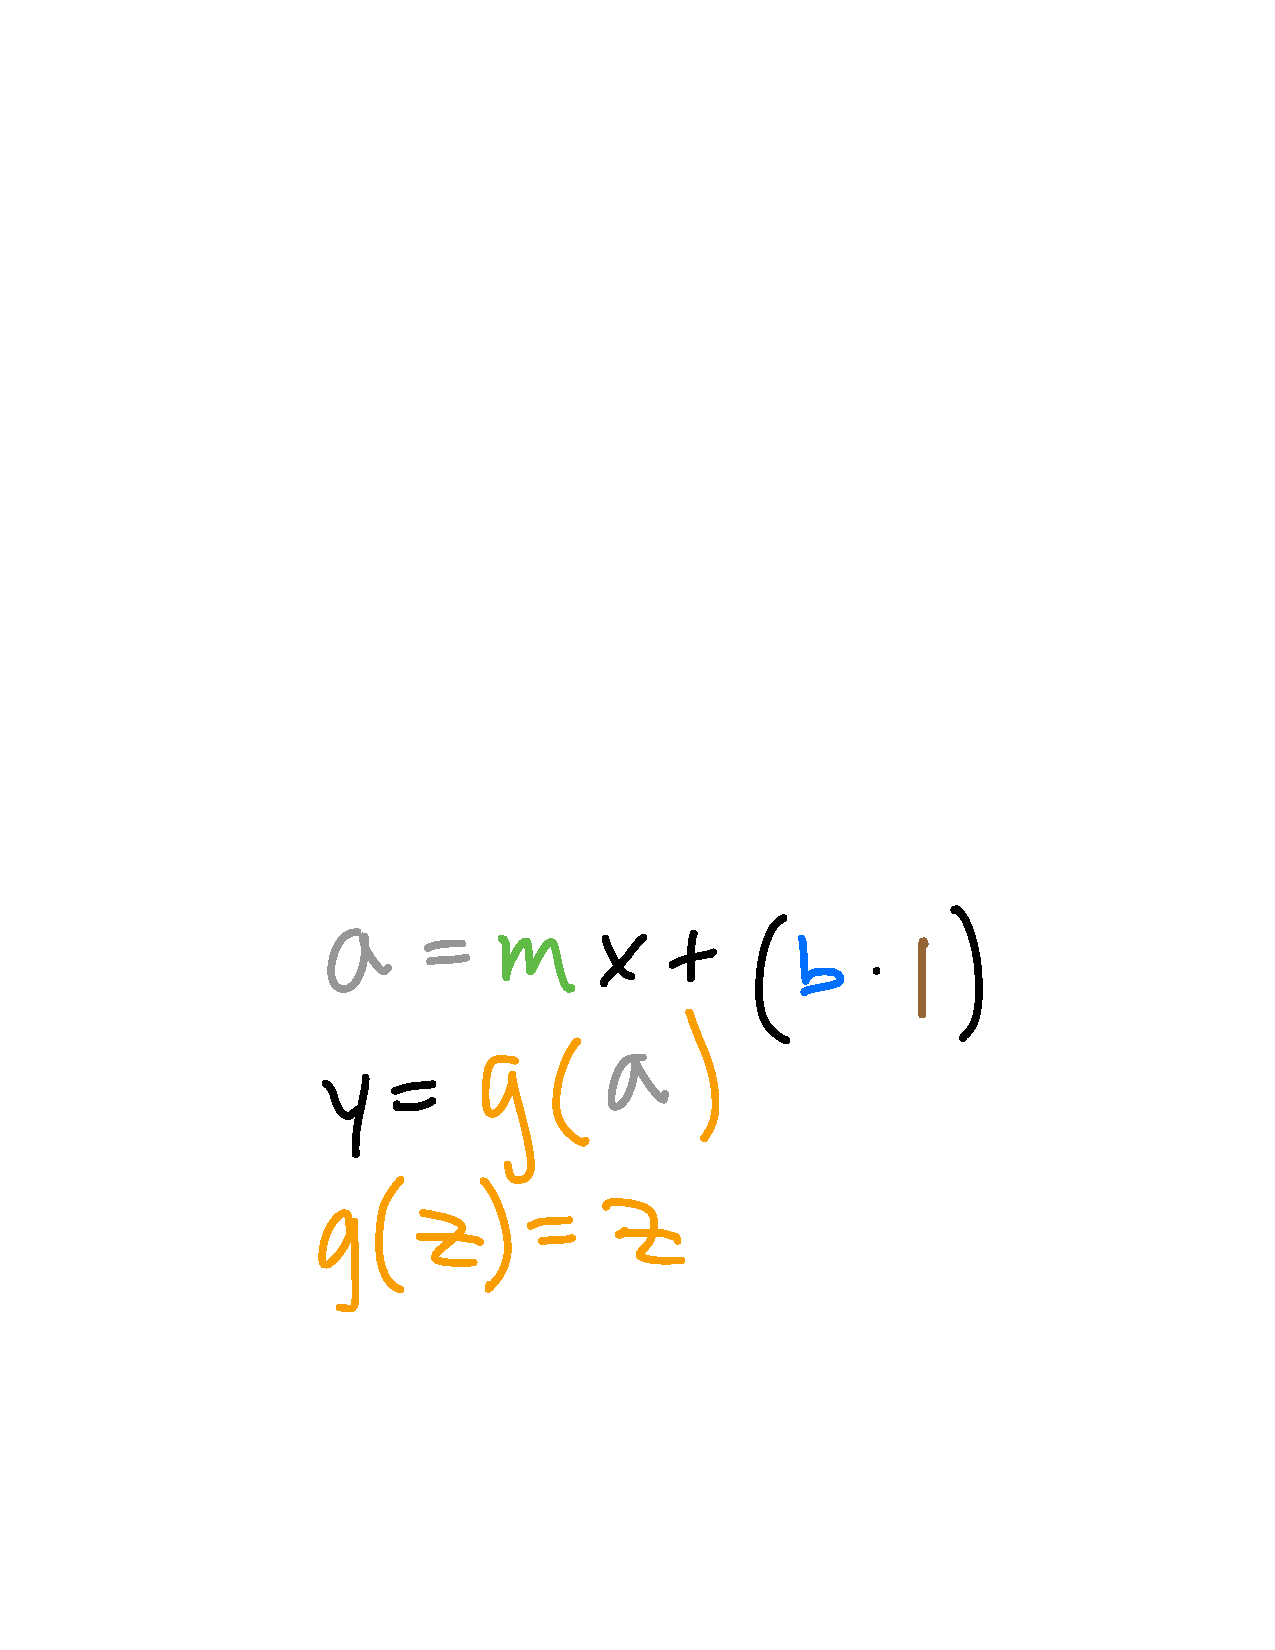
\includegraphics[width=0.50\textwidth]{./figures/lr_nn_2.pdf}
  \end{center}
\end{frame}

\begin{frame}{Linear regression using a neural network}
  \begin{center}
    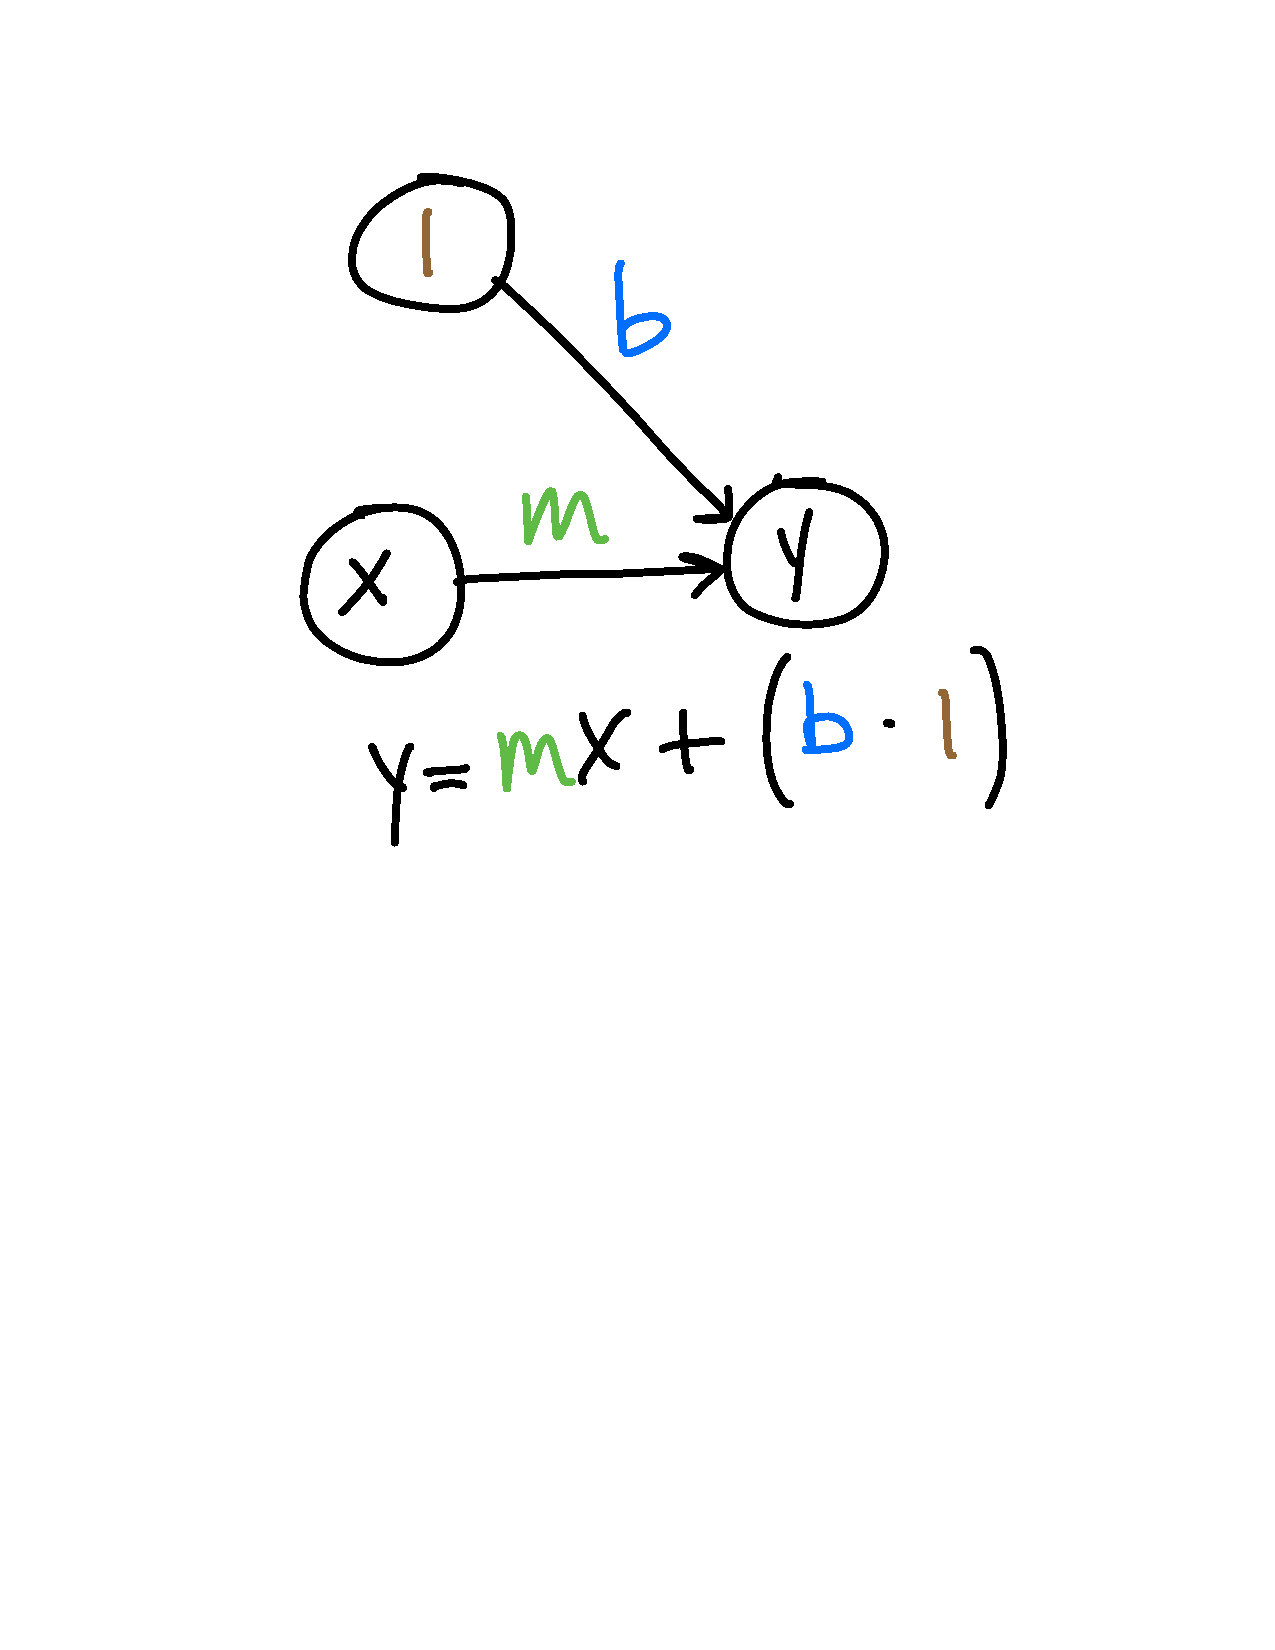
\includegraphics[width=0.50\textwidth]{./figures/lr_nn_1.pdf}
    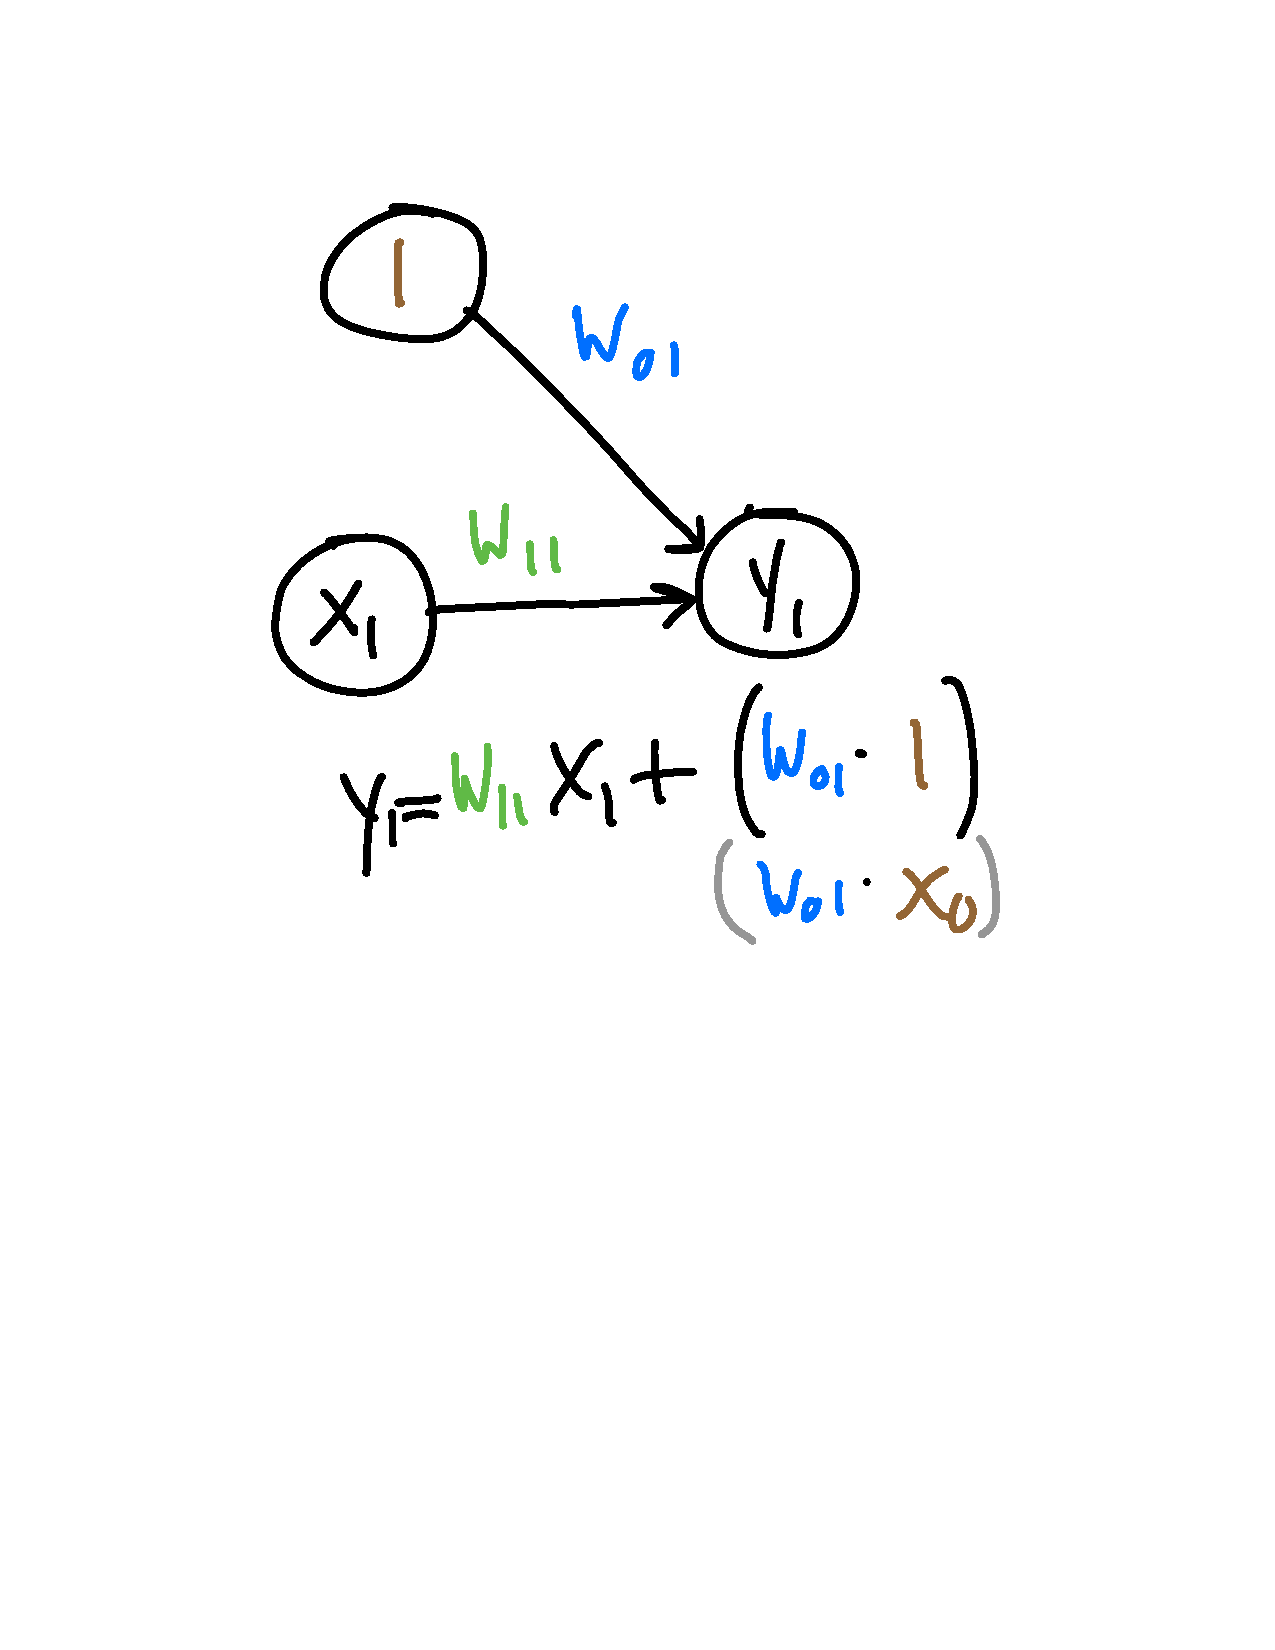
\includegraphics[width=0.50\textwidth]{./figures/lr_nn_3.pdf}
  \end{center}
\end{frame}

\begin{frame}{General architecture of neural networks}
  \begin{center}
    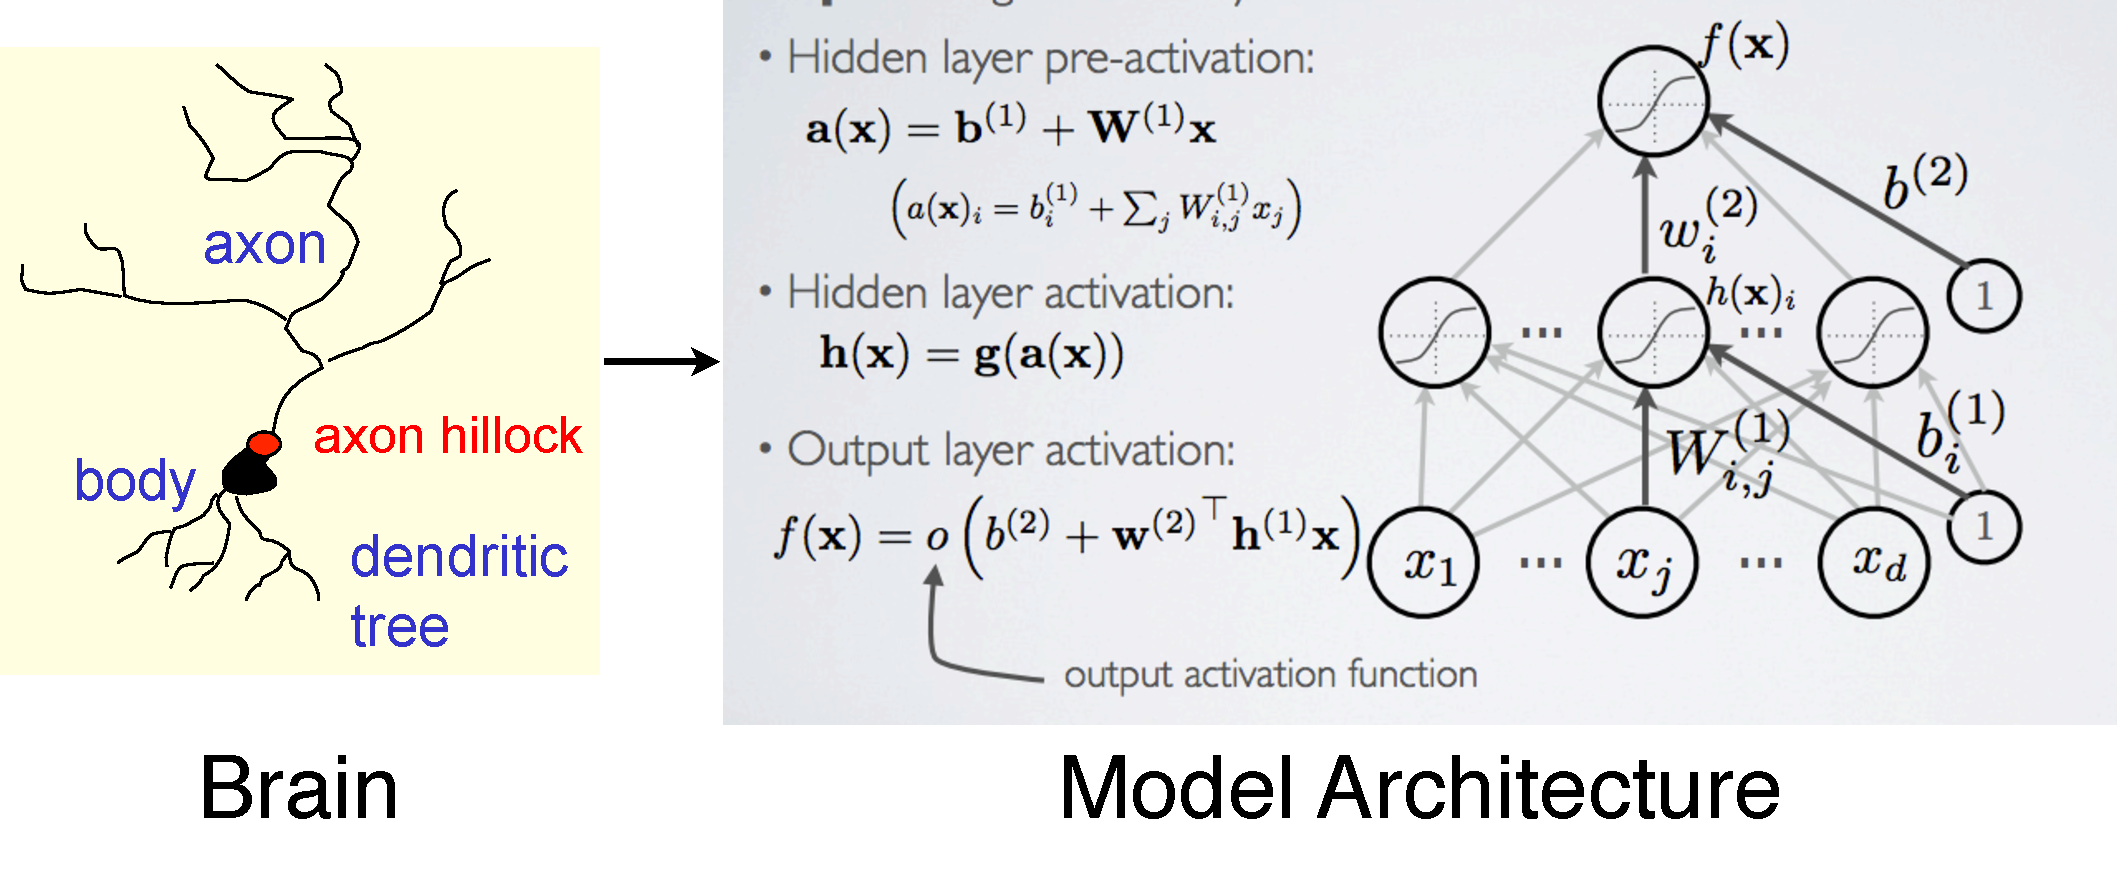
\includegraphics[width=1.00\textwidth]{./figures/brain_to_model.pdf}
  \end{center}
  Read from left \(\rightarrow\) right or bottom \(\rightarrow\) top.
\end{frame}

\begin{frame}{Neural networks perform nonlinear transformations}
  \begin{center}
    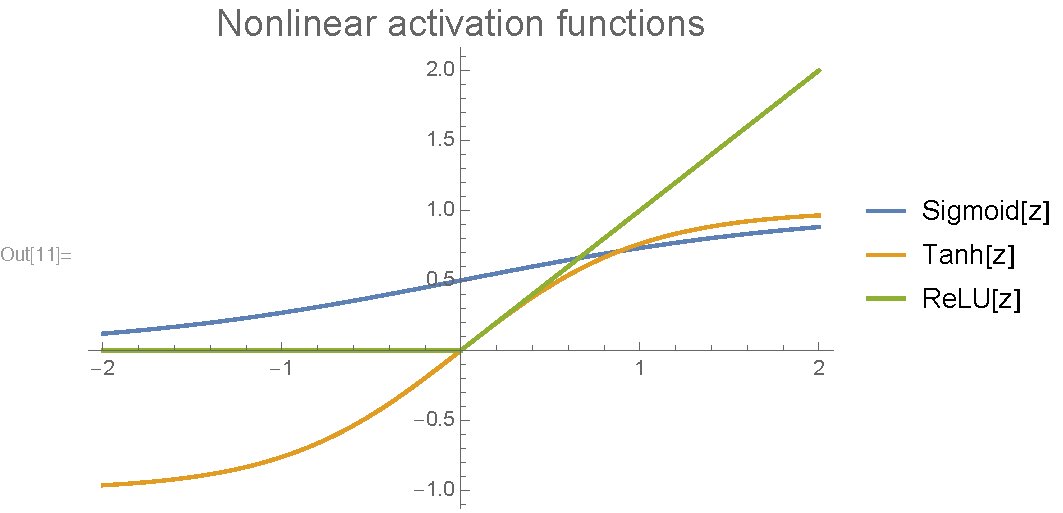
\includegraphics[width=1.00\textwidth]{./figures/nonlinear_activation.pdf}
  \end{center}
  The combination of hidden layers and nonlinear connections between layers makes them \emph{universal function approximators}.
\end{frame}

%% \begin{frame}{More complex neural networks}
%% \end{frame}

\begin{frame}{Training neural networks (placeholder)}
  \begin{center}
    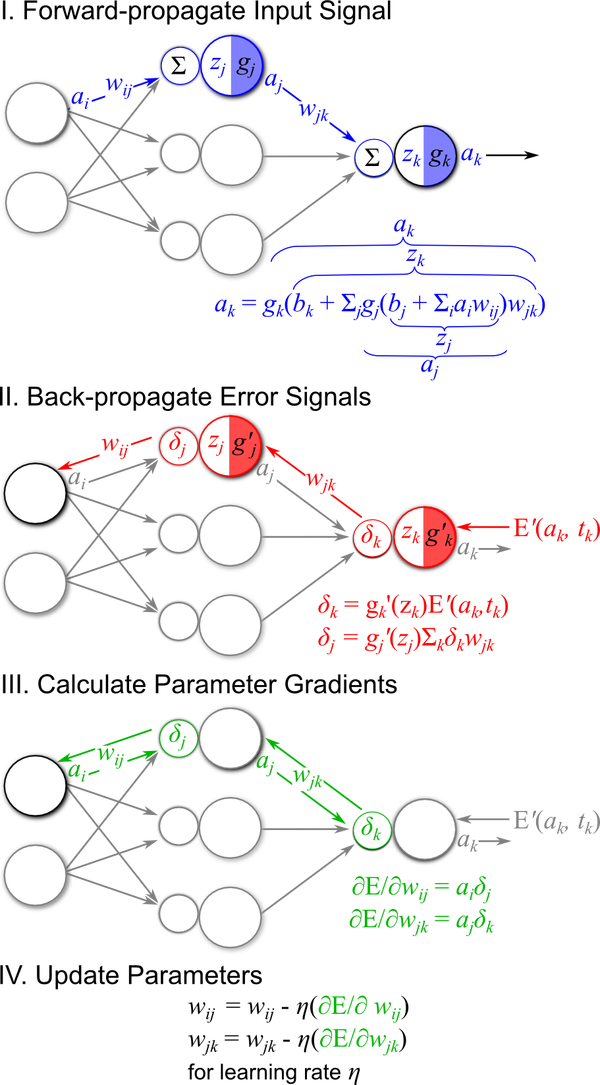
\includegraphics[width=0.50\textwidth]{./figures/fprop_bprop5.png}
  \end{center}
\end{frame}

\begin{frame}{An (imperfect) connection between neural networks and quantum chemistry}
  \begin{itemize}
  \item The fundamental components of the network (kind of neuron activation functions, convolution or direct connection) are like the \underline{Hamiltonian}, and
  \item the number of components in each network layer, the number of layers, and the input representation are like the size and type of \underline{basis set}.
  \end{itemize}
  Increasing the number of layers and number of nodes per layer is like lowering the variational bound of the network, and weights play a similar role to MO coefficients.
\end{frame}

\begin{frame}{The connection between basis sets and input featurization}
  What form the input of any ML model takes plays a large role on how well it performs.
  \begin{itemize}
  \item Adding diffuse functions to a basis set enables finding the correct (qualitative) answers for anions.
  \item Adding better input features (molecular descriptors) enables the model architecture to find better weights, leading to more accurate predictions.
  \end{itemize}
\end{frame}

\begin{frame}{Layer-wise Relevance Propagation (LRP)}
  \begin{center}
    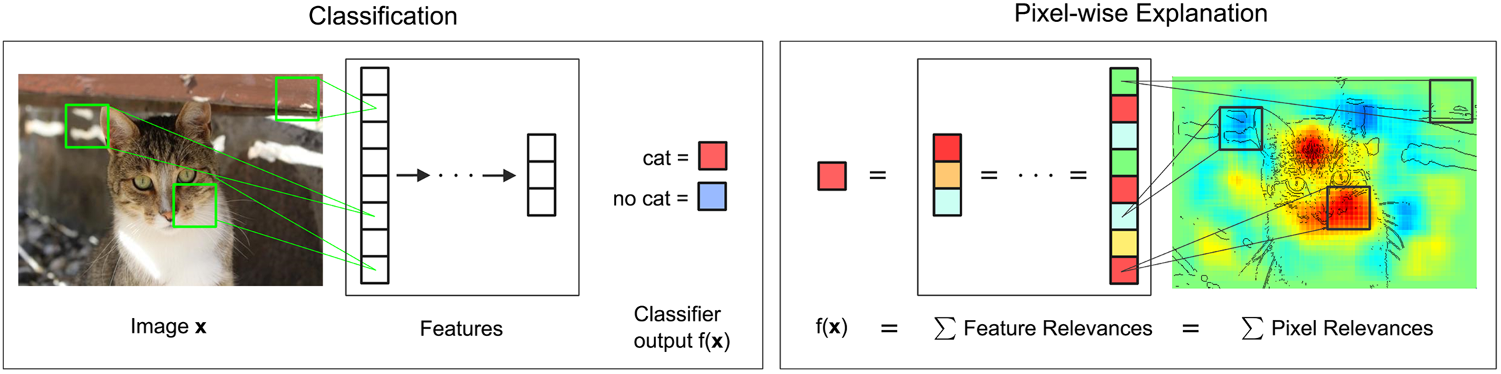
\includegraphics[width=1.00\textwidth]{./figures/2-Figure1-1.png}
  \end{center}
\end{frame}

\begin{frame}{LRP examples}
  \begin{center}
    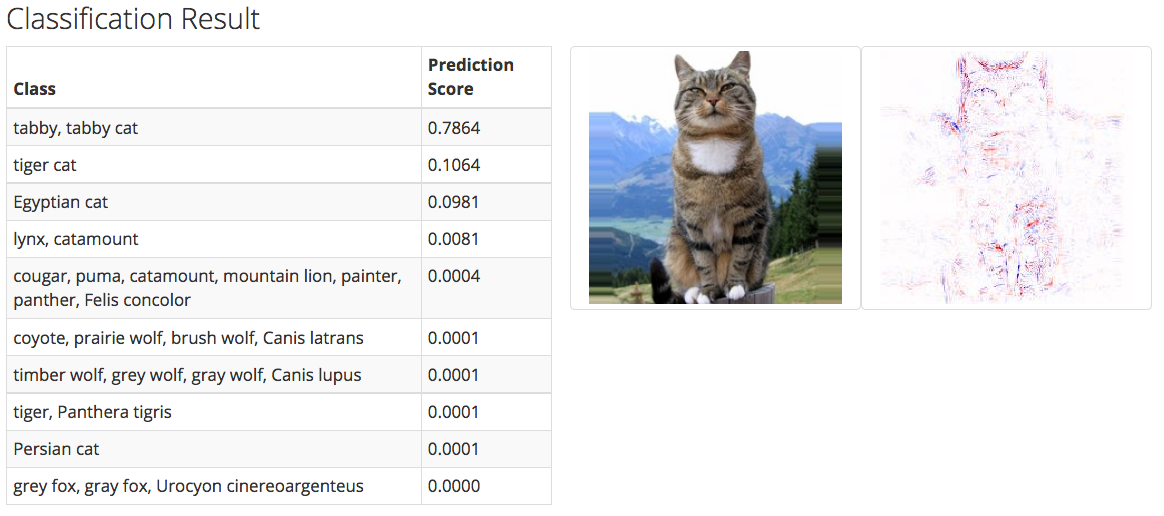
\includegraphics[width=1.00\textwidth]{./figures/lrp_example_1.png}
  \end{center}
\end{frame}

\begin{frame}{LRP examples}
  \begin{center}
    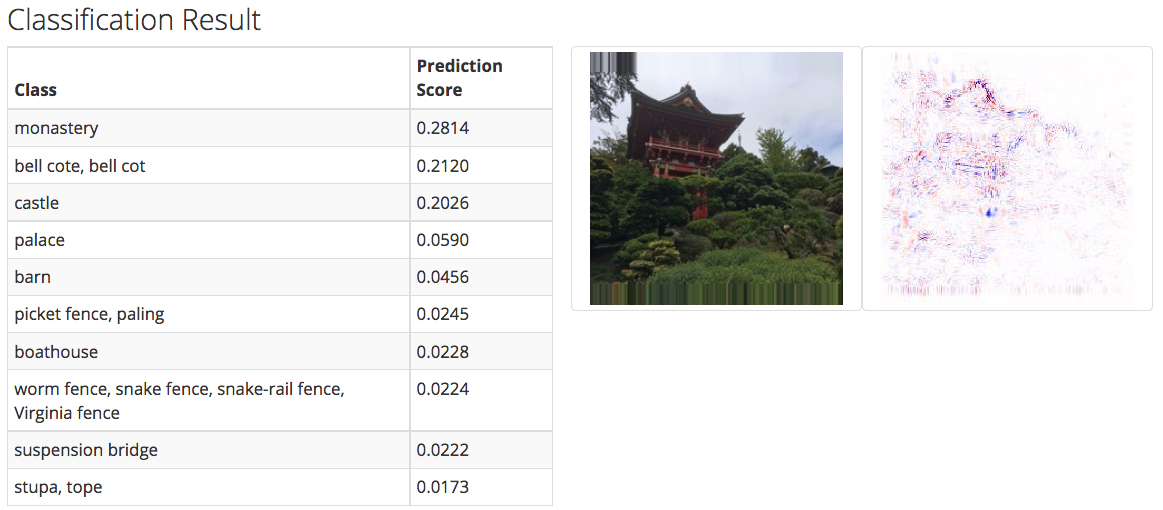
\includegraphics[width=1.00\textwidth]{./figures/lrp_example_2.png}
  \end{center}
\end{frame}

\begin{frame}{LRP examples}
  \begin{center}
    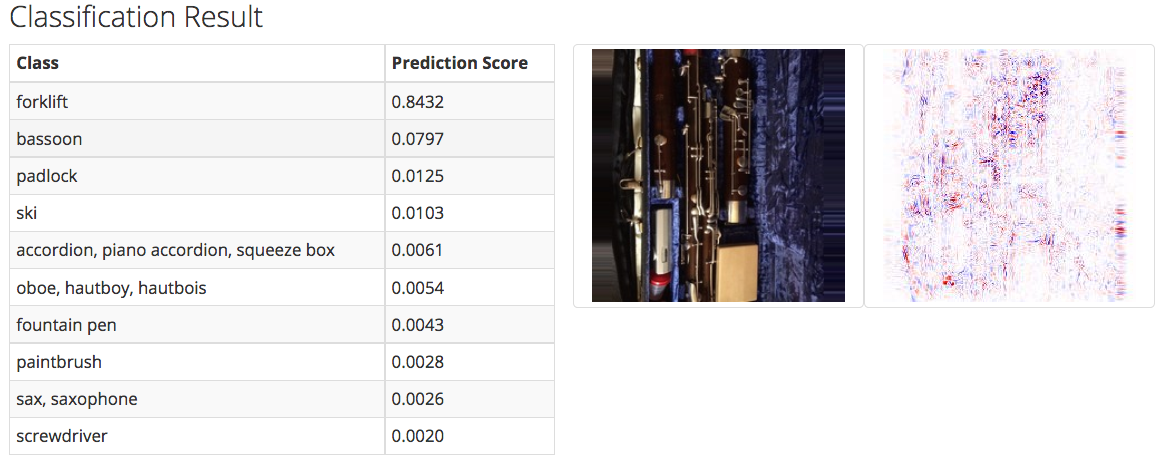
\includegraphics[width=1.00\textwidth]{./figures/lrp_example_3.png}
  \end{center}
\end{frame}

\begin{frame}{Learning the right thing for the right reason}
  \begin{center}
    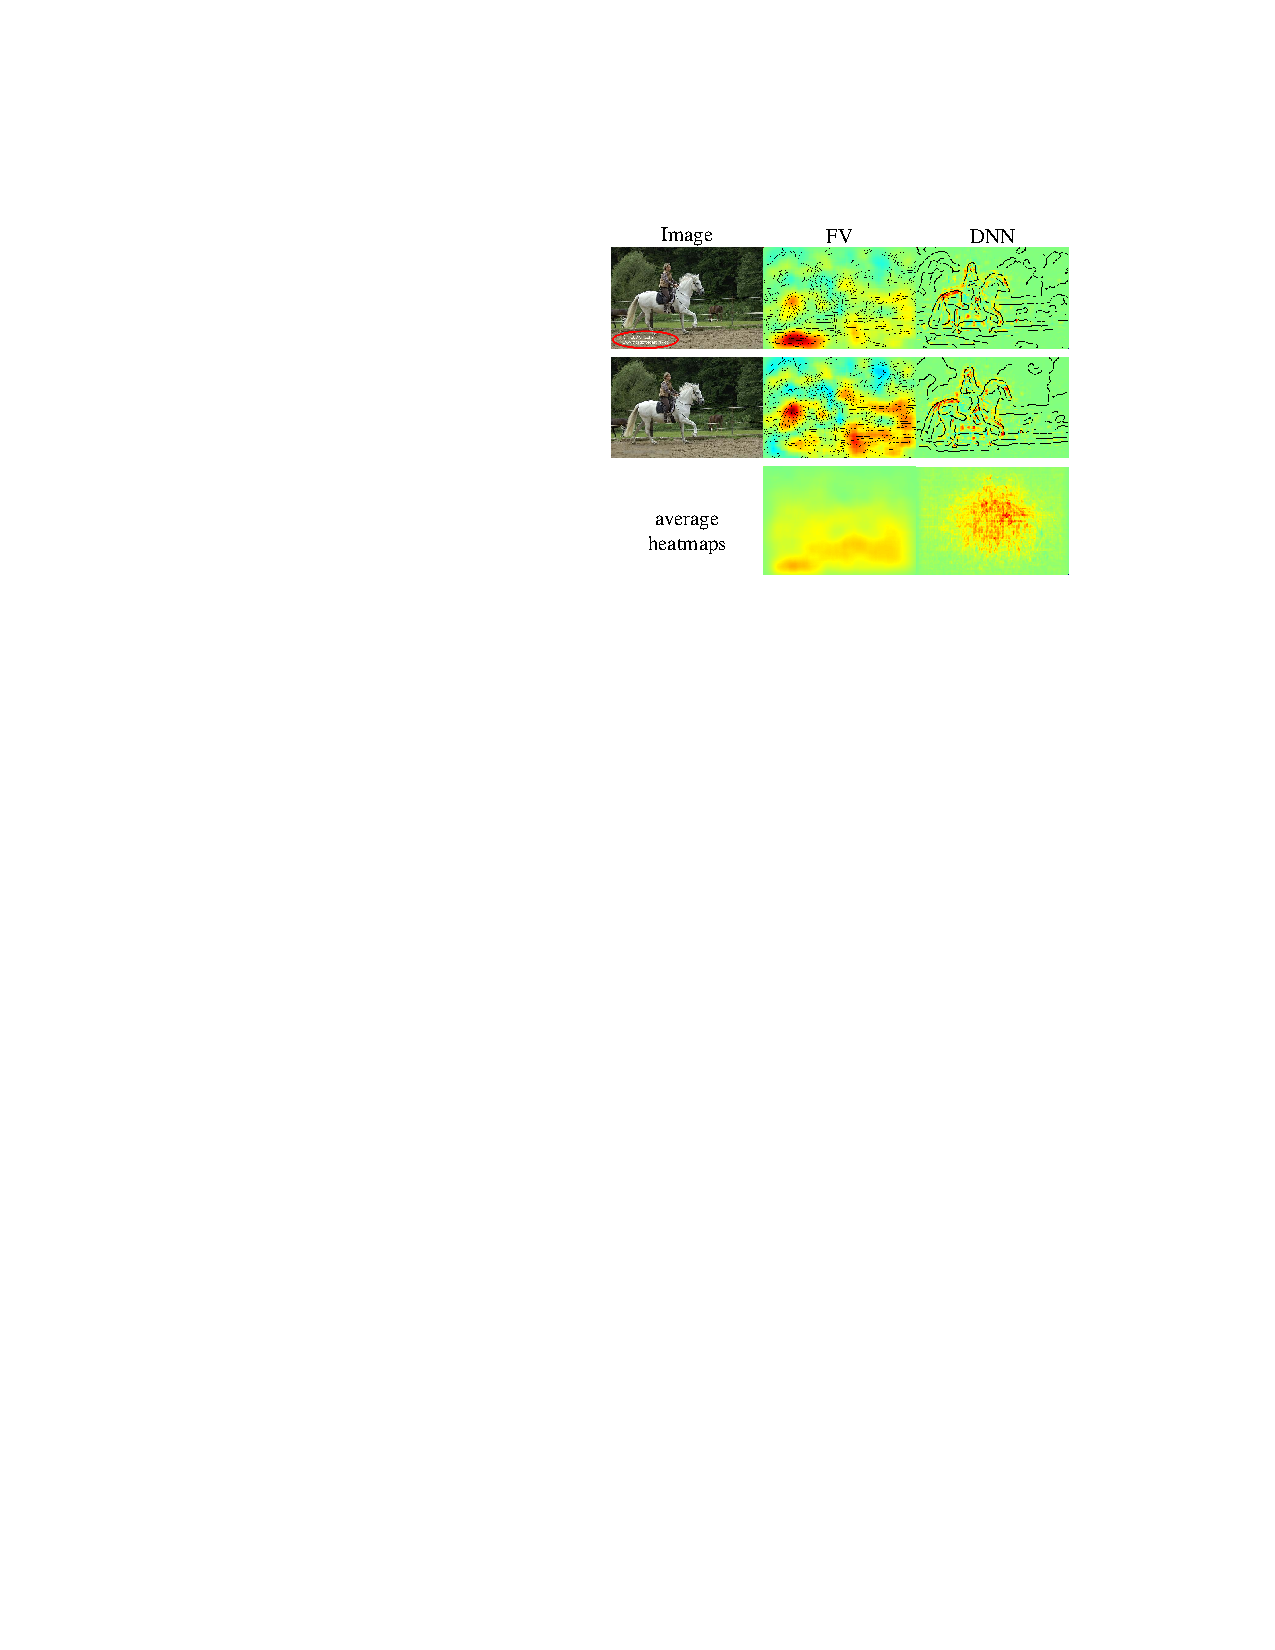
\includegraphics[width=1.00\textwidth]{./figures/fv_vs_dnn.pdf}
  \end{center}
\end{frame}

\begin{frame}{Aim \#1: Reproduction of Existing Literature Neural Networks}
  \begin{itemize}
  \item Discuss GC architecture, why choose GC architecture over DTNN, ANAKIN-ME, ...?
  \item Want comparison against literature results (more on this later), these so far are molecular energies only
  \item Where is the code?
  \item Why \emph{not} look at molecular energies? Want ML to do spectroscopy too, calculations for which are much more expensive than energies/trajectories.
  \end{itemize}
\end{frame}

\begin{frame}{Definitions of trained molecular properties}
  \begin{itemize}
  \item Zero-point (vibrational) energy: \(E_{\text{ZPVE}} = \frac{1}{2} h \sum_{i}^{\text{normal modes}} \nu_{i}\)
  \item Isotropic polarizability (static, \(\omega = 0\)): \(\alpha_{\text{iso}} = \bar{\alpha} \equiv \frac{1}{3} (\alpha_{xx} + \alpha_{yy} + \alpha_{zz})\)
  \end{itemize}
\end{frame}

\begin{frame}{Aim \#2: Characterization of Existing Literature Neural Networks}
  \begin{itemize}
  \item Math w/ example pictures
  \item Expected outcomes
  \end{itemize}
\end{frame}

\begin{frame}{Relationship between feed-forward pass and LRP pass}
  \begin{center}
    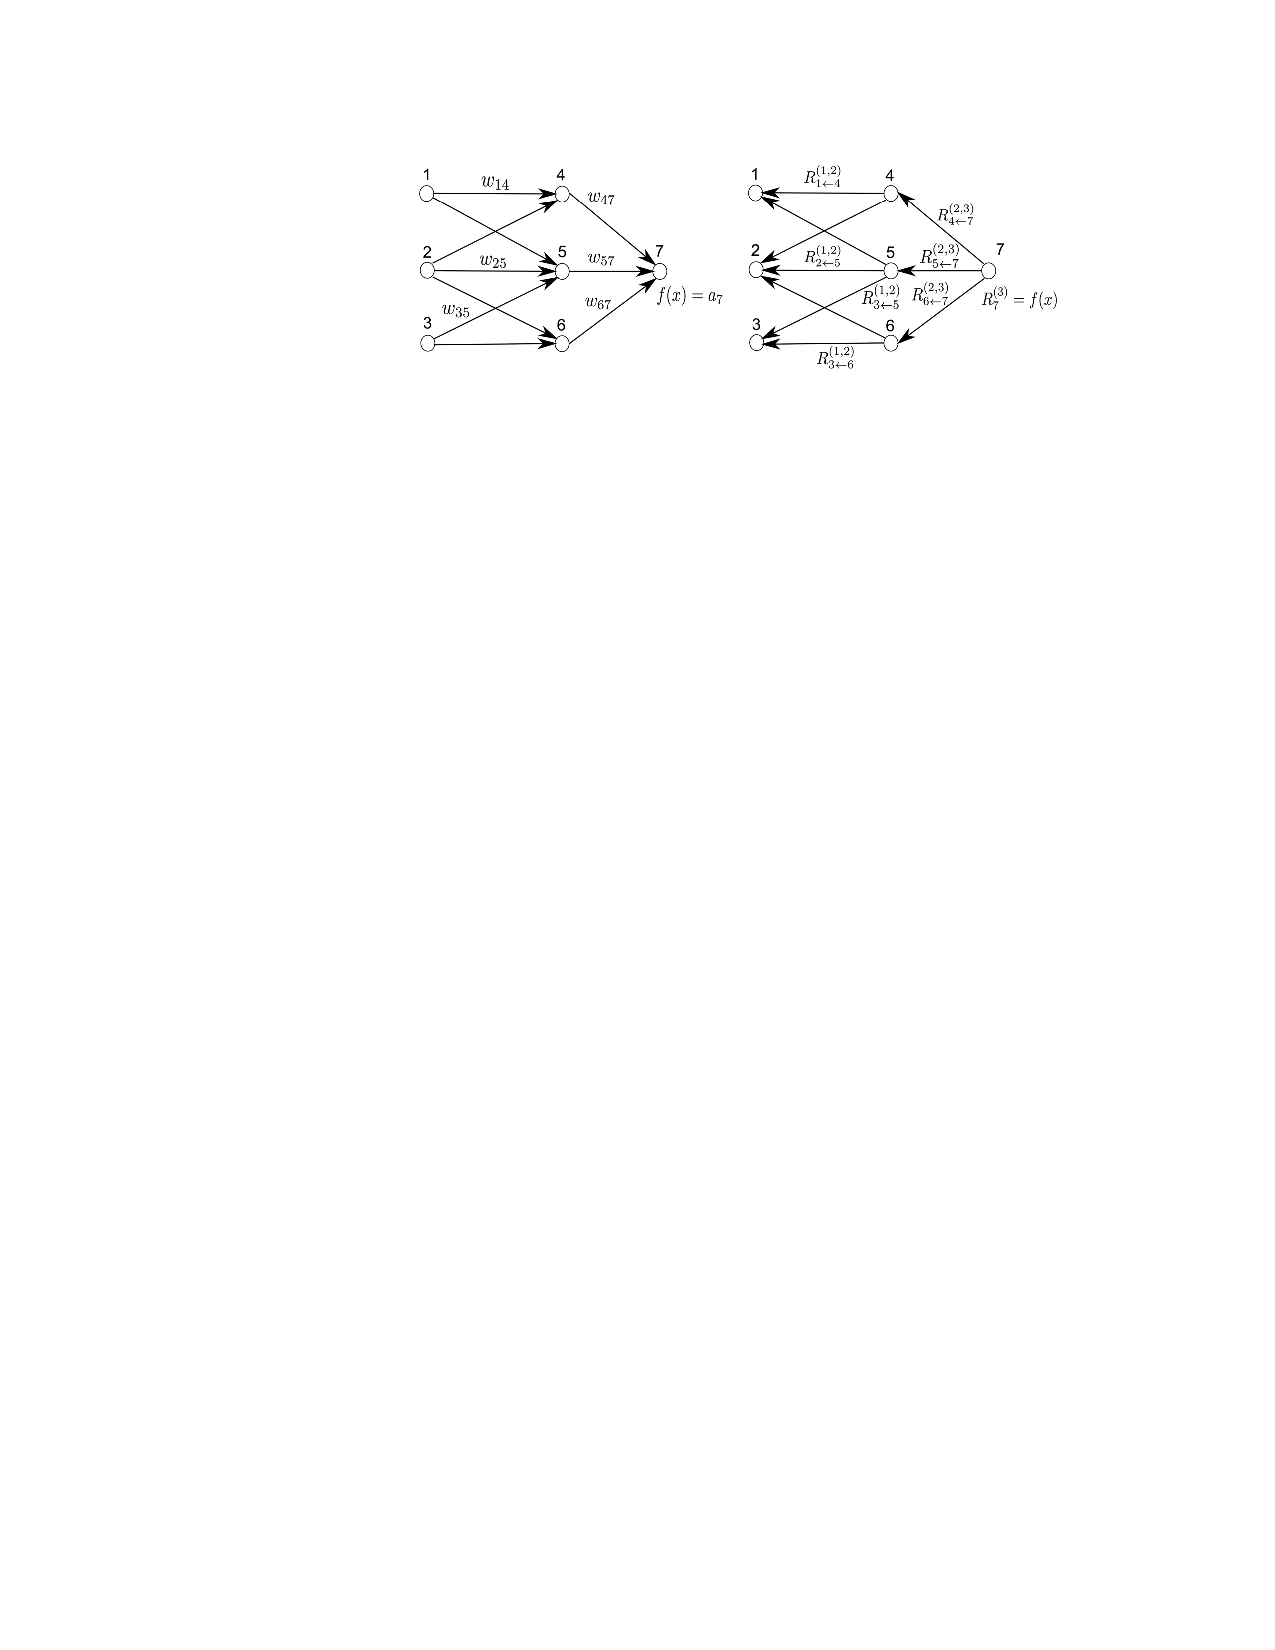
\includegraphics[width=1.05\textwidth]{./figures/fig2_trimmed.pdf}
  \end{center}
\end{frame}

\begin{frame}{What LRP is \protect\emph{not} doing}
  \begin{itemize}
    \item This is \emph{not} a direct inspection of what the NN has learned!
    \item Looking directly at NN weights is like looking at MO coefficients. Once the number of them grows, the ``importance'' of a single one diminishes greatly, and the number of nodes/weights grows even quicker than the number of MO coefficients for a reasonable quantum chemical calculation. The ability for direct inspection becomes impossible.
    %% \item Toy models are unlikely to be useful for any kind of understanding the effect of chemical data on NNs because of the complexity of \emph{any} molecule compared to NNs. In a way, a toy or model molecule w/ an \textit{ab initio} calculation can give more insight than a model NN. We are asking NN parameters to be both more efficient and more general than MO coefficients at describing the many-particle wavefunction!
  \end{itemize}
\end{frame}

%% most likely diminishes greatly. If one is particularly important, how to identify it? Do the weights form a distribution that can be inspected?

\begin{frame}{A better analogy}
  %% between relevance propagation and interaction energy decomposition approaches (SAPT, EDA):
  The use of layer-wise relevance propagation is identical to intermolecular interaction energies.
  \begin{itemize}
  \item SAPT and ALMO-EDA give the best theoretical, physically-intuitive, and \emph{quantitative} insight into how molecules interact.
  \end{itemize}
\end{frame}

\begin{frame}{}
  \begin{center}
    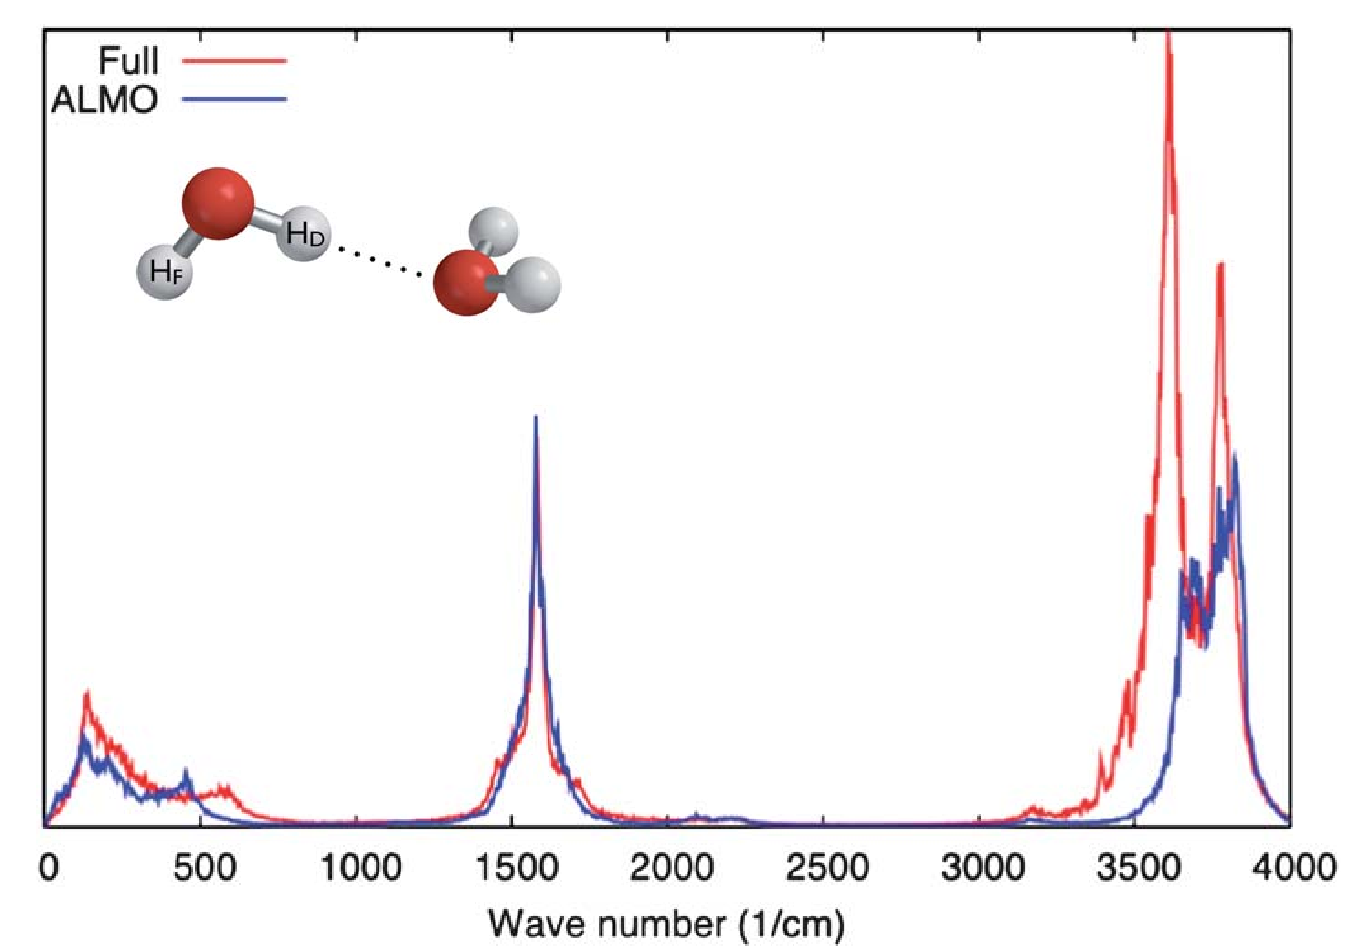
\includegraphics[scale=0.50]{./figures/almo_water_combined.pdf}
  \end{center}
\end{frame}

\begin{frame}{}
  \begin{center}
    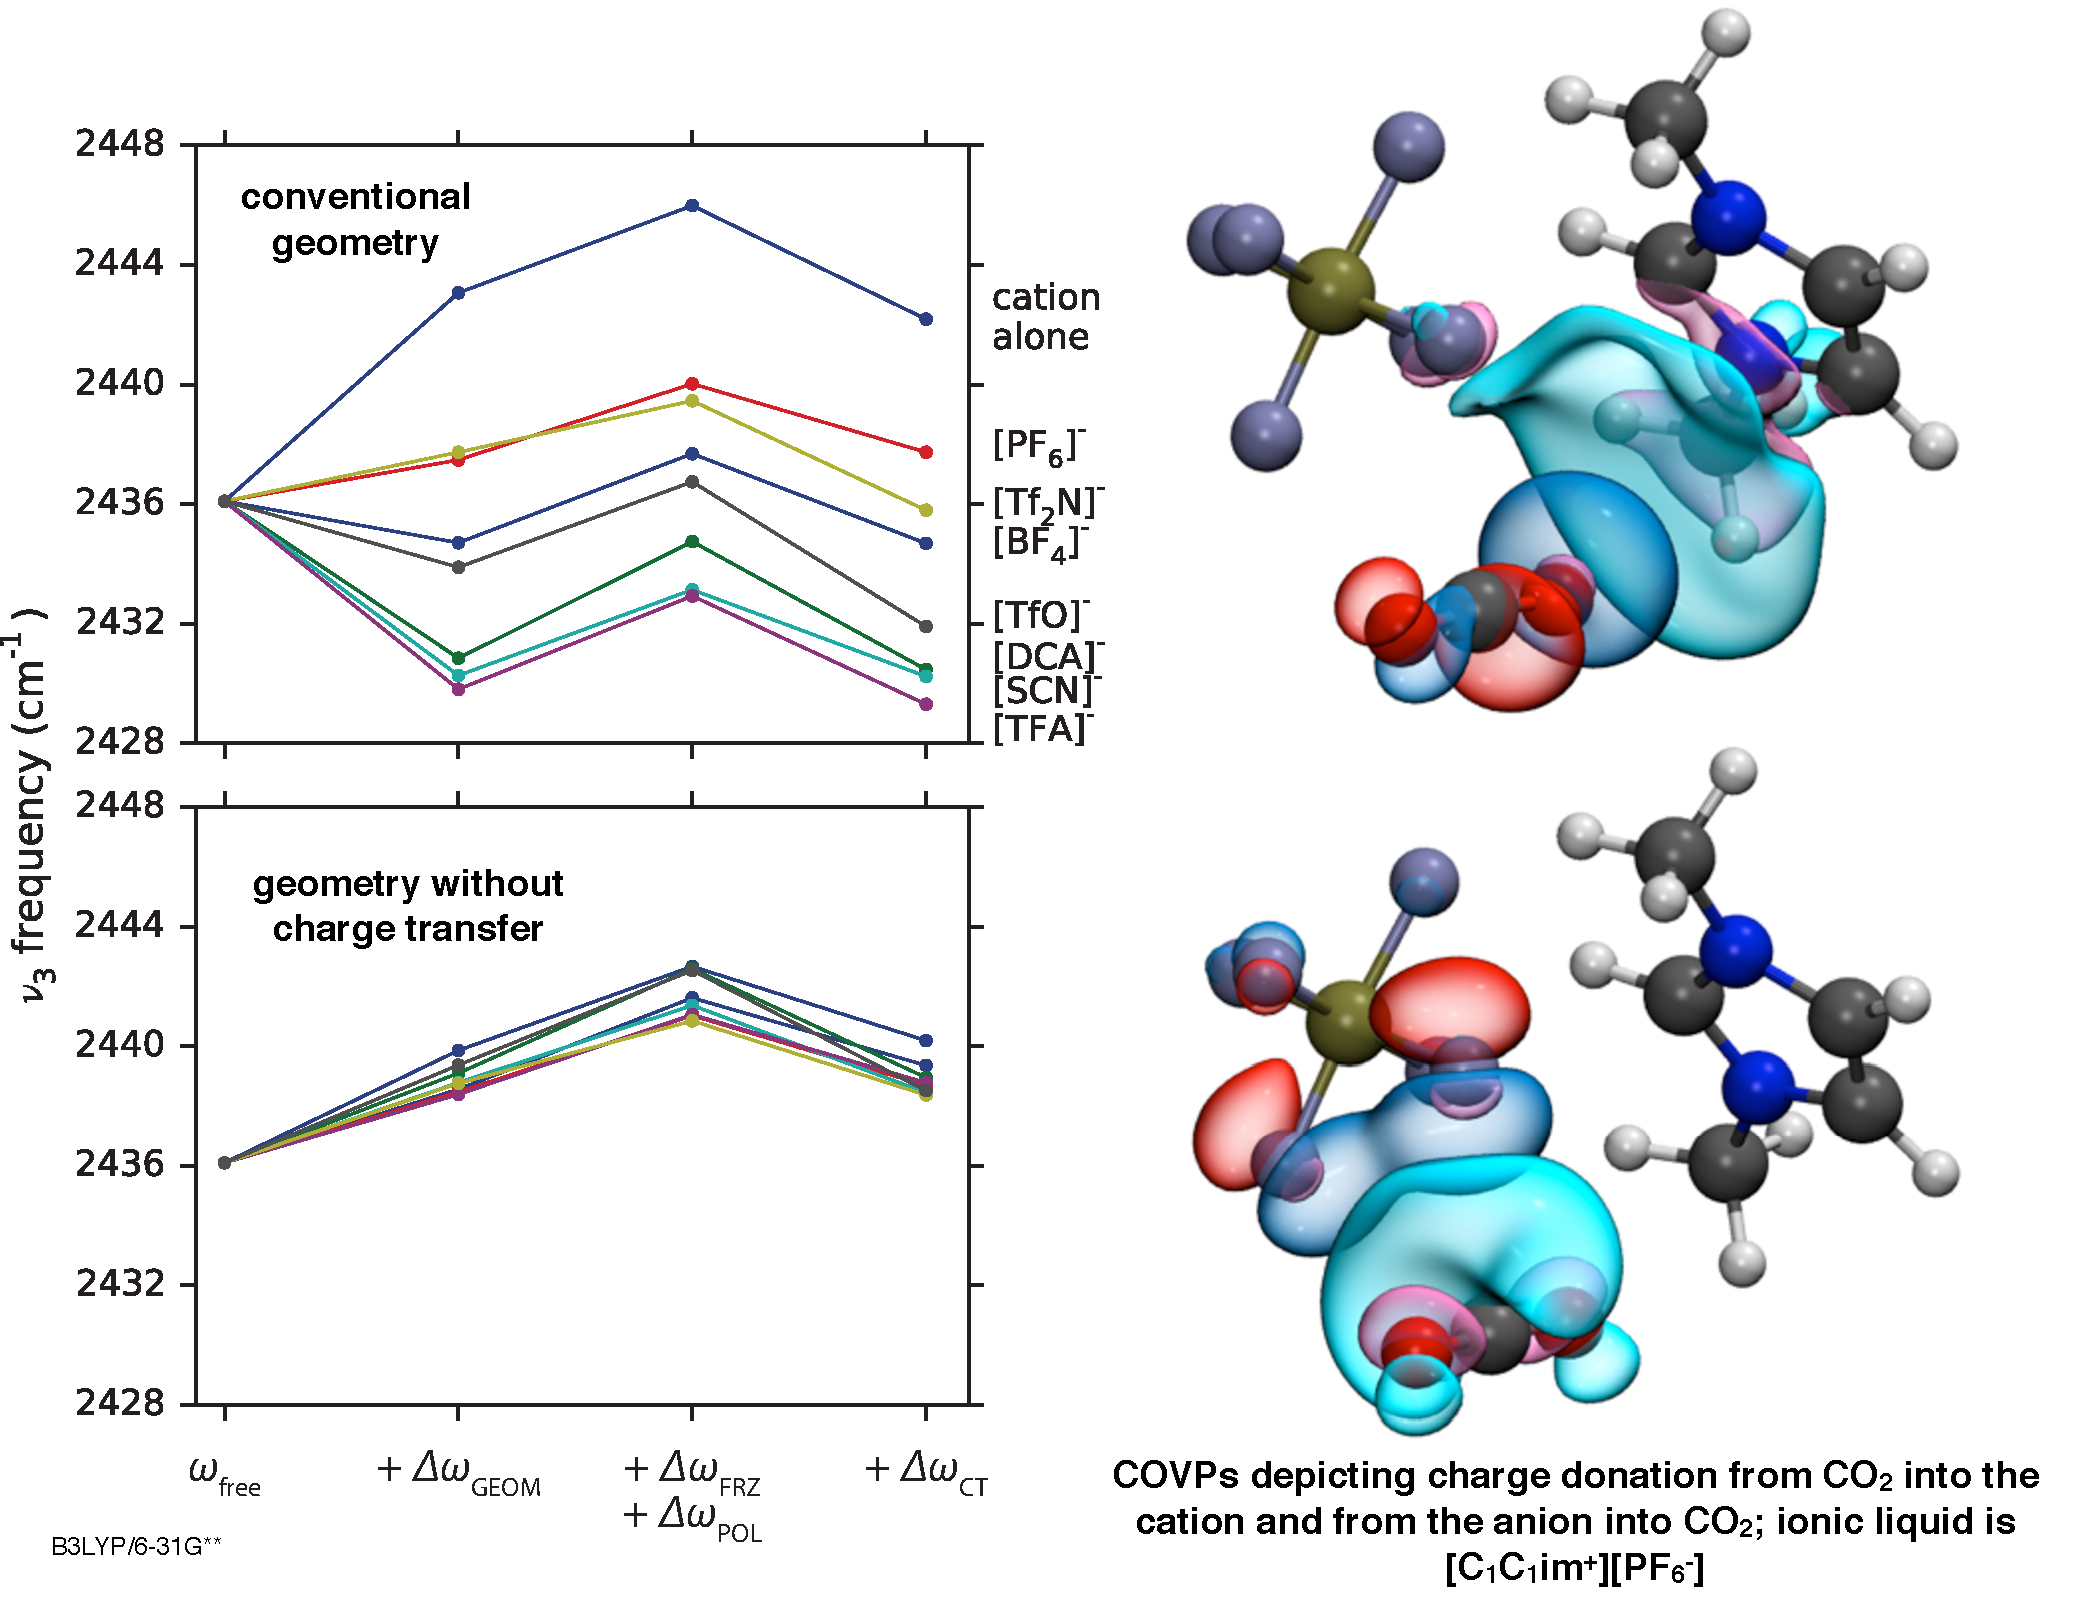
\includegraphics[scale=0.30]{./figures/slide_ionic_liquid.pdf}
  \end{center}
\end{frame}

%% How does LRP prove that a NN is transferable?

\begin{frame}{Aim \#3: Training Neural Networks for Complex Molecular Properties}
  \begin{itemize}
  \item What are the properties, logic behind the choice
  \item Expected outcomes
  \end{itemize}
\end{frame}

\begin{frame}{Definitions of trained molecular properties}
  \begin{itemize}
  \item Zero-point (vibrational) energy: \(E_{\text{ZPVE}} = \frac{1}{2} h \sum_{i}^{\text{normal modes}} \nu_{i}\)
  \item Isotropic polarizability (static, \(\omega = 0\)): \(\alpha_{\text{iso}} = \bar{\alpha} \equiv \frac{1}{3} (\alpha_{xx} + \alpha_{yy} + \alpha_{zz})\)
  \item Parallel 1st hyperpolarizability (static, \(\omega_{a} = \omega_{b} = 0\)): \(\beta_{\parallel} = \frac{3}{5|\mu|} \sum_{i,j=x,y,z} \beta_{iij} \mu_{j}\)
  \item All vibrational frequencies: \(\{\tilde{\nu}\}_{\text{normal modes}}\)
  \end{itemize}
\end{frame}

\begin{frame}{Aim \#4: Characterization of Novel Neural Networks}
  \begin{itemize}
  \item Unsupervised learning (PCA analogy)
  \item Denoising autoencoder
  \item Expected outcomes
  \end{itemize}
\end{frame}

\begin{frame}{Learning a compressed representation}
  \begin{center}
    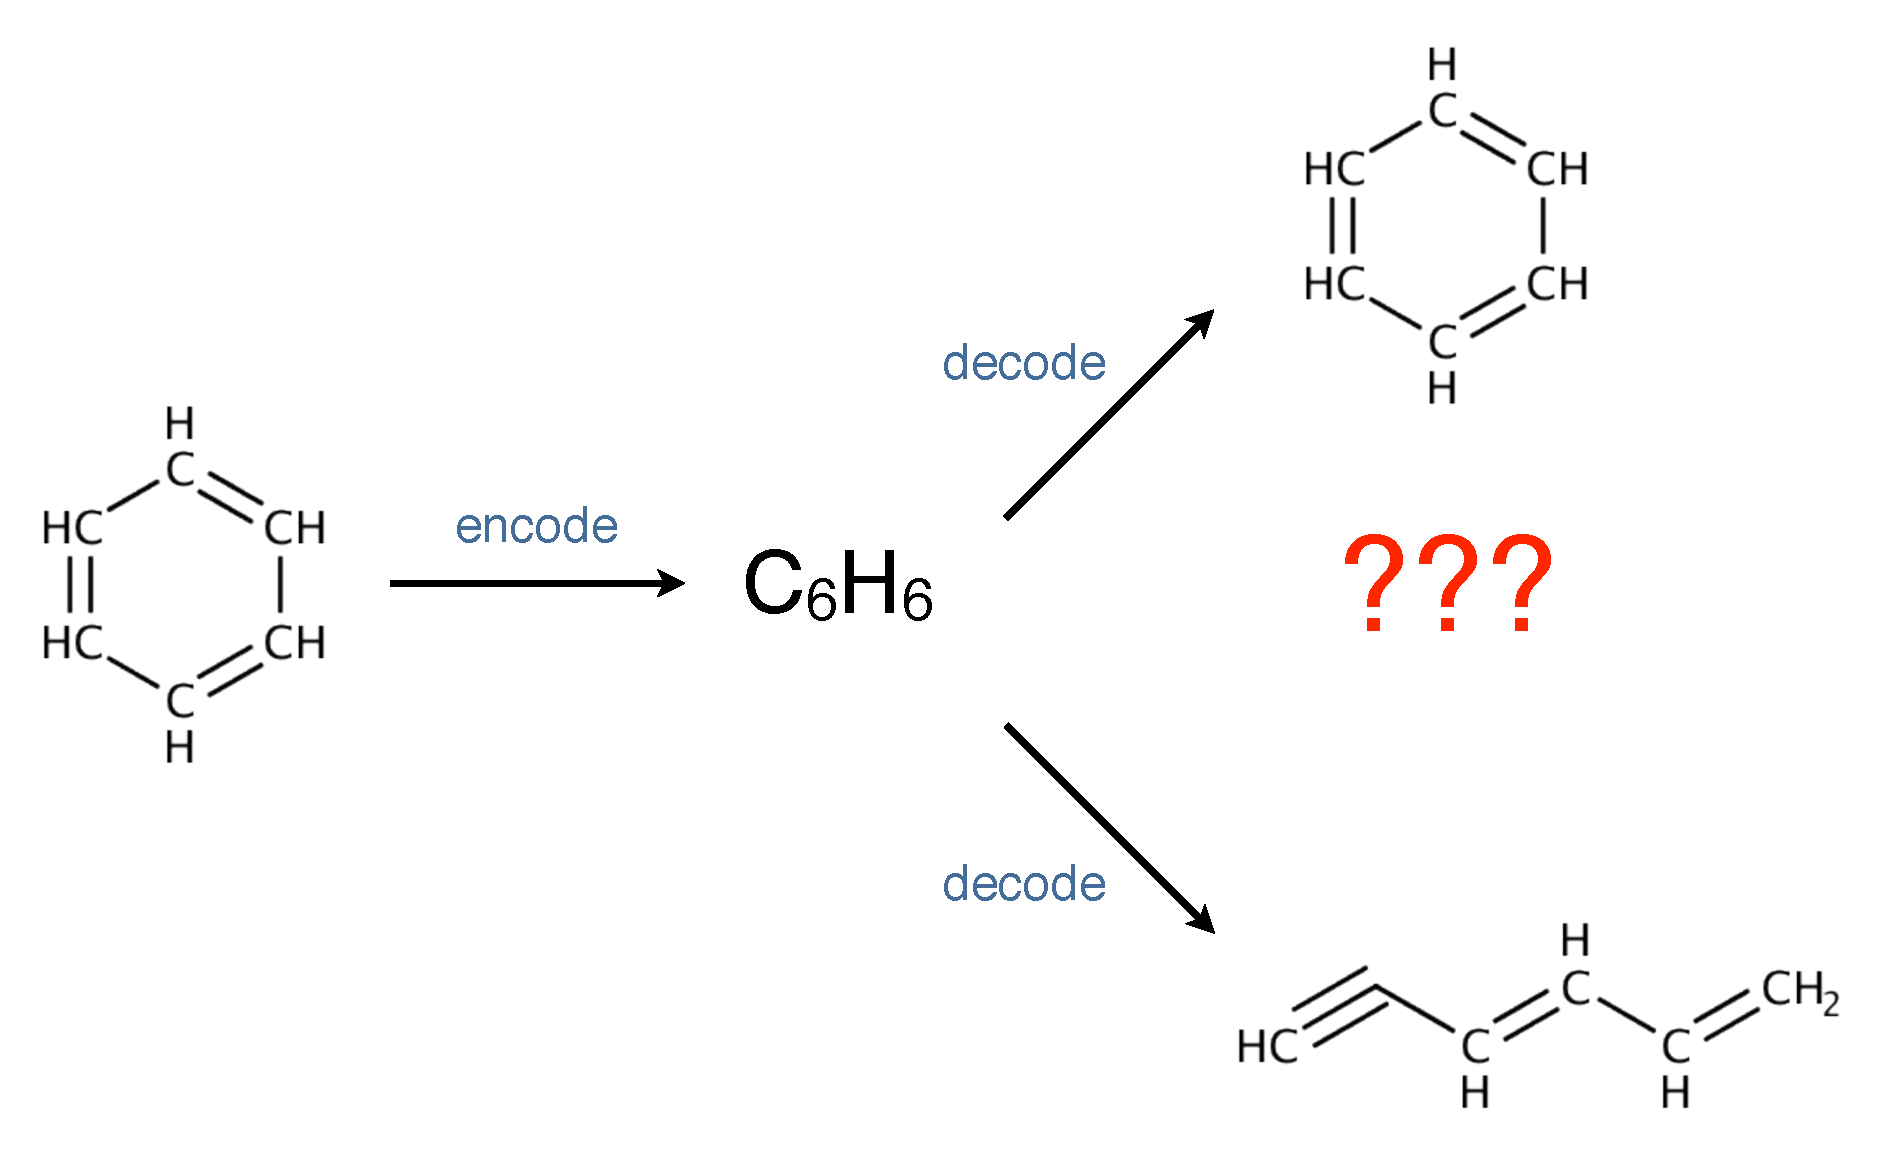
\includegraphics[width=1.00\textwidth]{./figures/autoencoder_example.pdf}
  \end{center}
  Attempt to reduce some complex input into a smaller form (code) that can accurately be turned back into the complex input
\end{frame}

\begin{frame}{Autoencoder structure}
  \begin{center}
    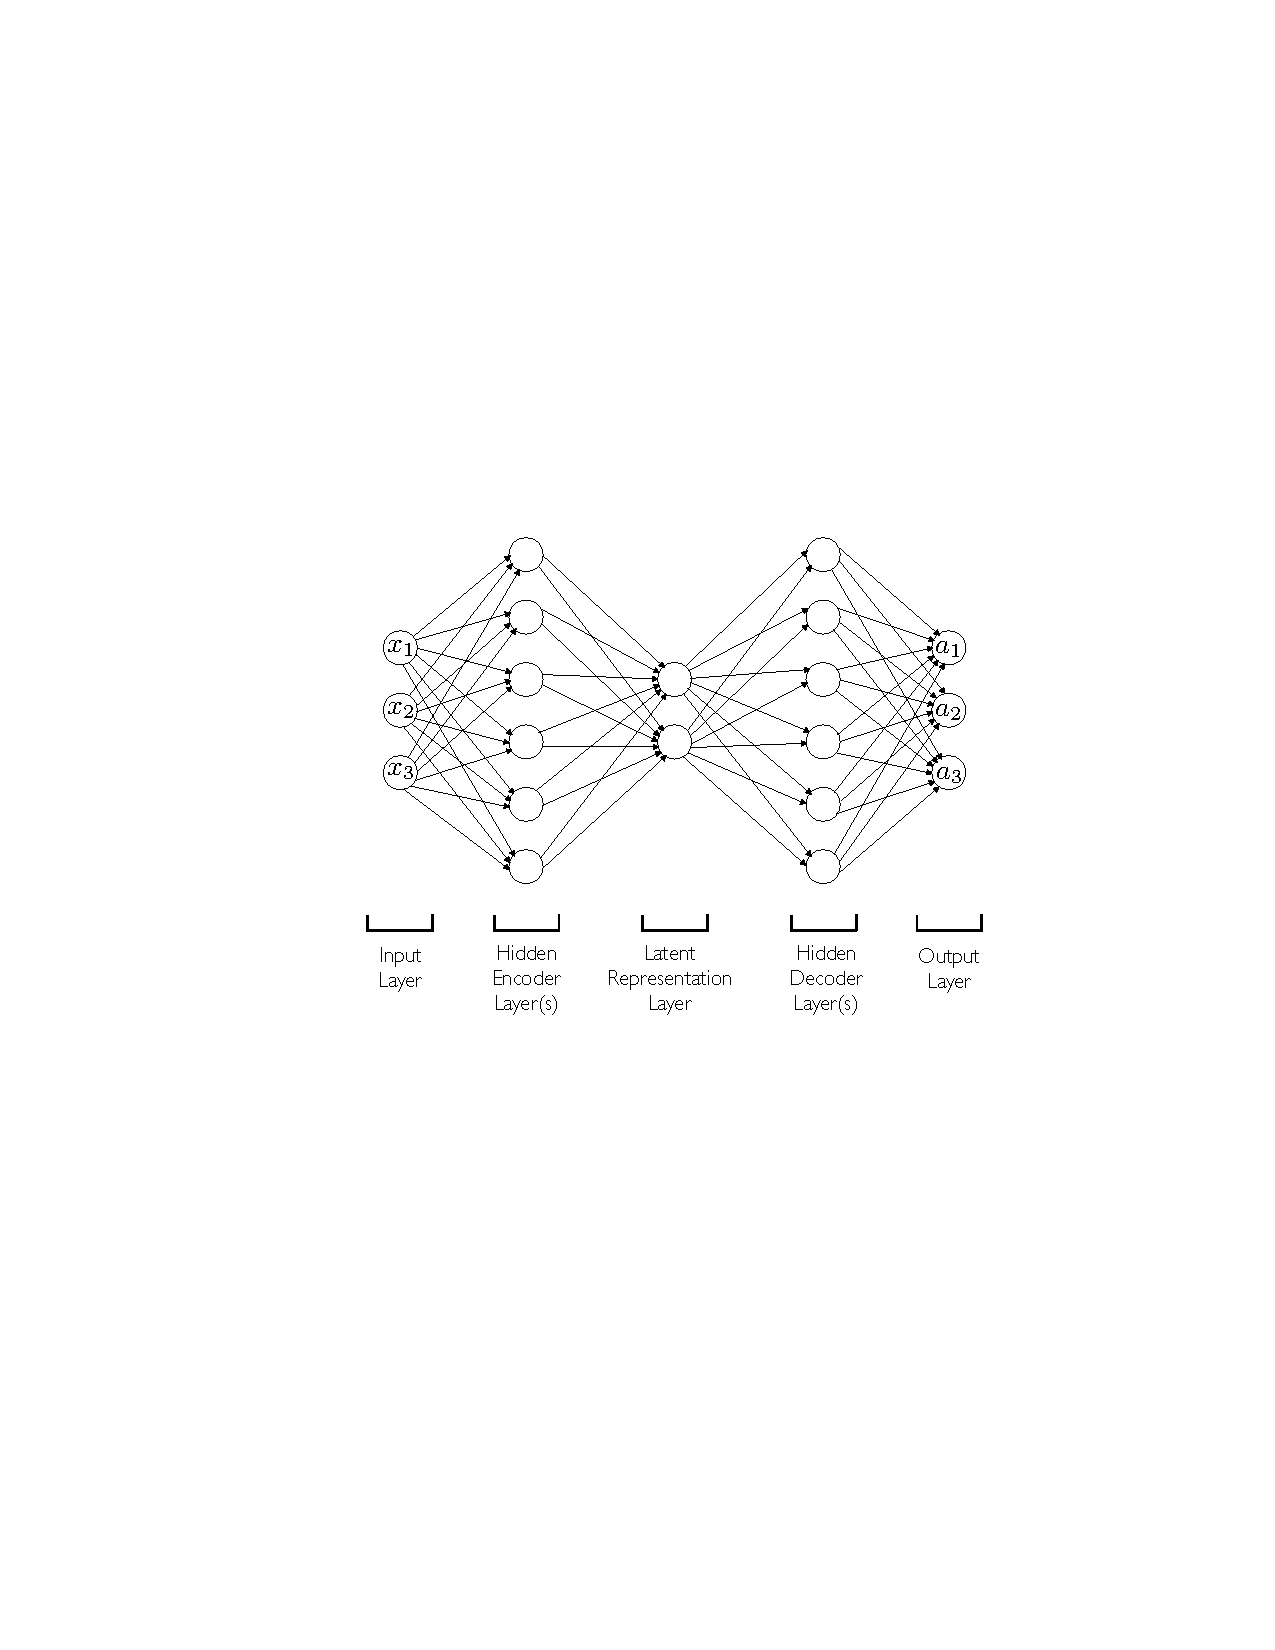
\includegraphics[width=0.80\textwidth]{./figures/autoencoder.pdf}
  \end{center}
  A \textit{denoising} autoencoder adds noise to the input during training.
\end{frame}

\begin{frame}{Approximate Timeline}
\begin{table}[]
\centering
\begin{tabular}{@{}rp{0.55\textwidth}l@{}}
\toprule
Specific Aim & Task                                    & \# of Months \\ \midrule
1            & code development: forming pipeline      & 3            \\
1            & model training                          & 2            \\
2            & code development: adapt LRP to pipeline & 3            \\
2            & analysis development                    & 2            \\
3            & hyperpolarizability calculations        & 2            \\
3            & model training                          & 3            \\
4            & code development: DAE                   & 2            \\
4            & model training                          & 2            \\
4            & analysis                                & 2            \\ \midrule
Total        &                                         & 21           \\ \bottomrule
\end{tabular}
\end{table}\end{frame}

\begin{frame}{Backup Slides}
\end{frame}

\begin{frame}{A future challenge: building databases}
  \begin{itemize}
  \item GDB9/QM9 is the most commonly-used training set, the equivalent of the MNIST set of \textasciitilde{}10,000 labeled handwritten digits.
  \item It is now suffering from the same problem as MNIST: it is too simple and not representative of real-world training cases (molecules).
  \item Analogy: Pople basis sets (6-31G and derivatives) are still extremely common, not even because we don't know better, but because we ``need to compare to past work''.
  \item If a \emph{general and transferable} ML model fails on GDB9, that is a warning sign, but the above cannot be a reason against extending deeper into chemical space for ML model training.
  \end{itemize}
\end{frame}

\begin{frame}{Hyperpolarizability equations from paper}
  When the dipole moment coincides with the \(j\)-axis, we have
  \begin{equation}
    \beta_{\parallel} = \frac{3}{5}\beta_j = \frac{1}{5} \sum_{i=x,y,z} (\beta_{iij} + \beta_{iji} + \beta_{jii}),
  \end{equation}
  or in the general case,
  \begin{equation}
    \beta_{\parallel} = \frac{3}{5|\mu|} \sum_{i,j=x,y,z} \beta_{iij} \mu_{j},
  \end{equation}
  where
  \begin{equation}
    \beta_{ijk} = \left<\left<\mu_{i};\mu_{j},\mu_{k}\right>\right>.
  \end{equation}
\end{frame}

\begin{frame}{What is a ``one-hot'' vector?}
  \begin{quote}
    (...) a group of bits among which the legal combinations of values are only those with a single high (1) bit and all the others low (0).
  \end{quote}
  For a variable that can take a finite set of \(n\) values, it can be represented as binary vector of length \(n\).
  \begin{table}[htbp]
    \centering
    \begin{tabular}{@{}lll@{}}
      \toprule
      Feature & Description & Size \\ \midrule
      Atom type & H, C, N, O, or F (one-hot) & 5 \\ \bottomrule
    \end{tabular}
  \end{table}
  If atom type is the first feature, this is the third atom in the input, and the element is oxygen, then \(x_{1}^{(3)} = (0, 0, 0, 1, 0)\).
\end{frame}

%% \begin{frame}{Convolution}
%%   Mathematical form:
%%   \begin{align}
%%     (f * g)(t) &= \int_{-\infty}^{\infty} f(\tau) g(t-\tau) \,d\tau \\
%%                &= \int_{-\infty}^{\infty} f(t-\tau) g(\tau) \,d\tau
%%   \end{align}
%%   In the context of a neural network:
%% \end{frame}

\begin{frame}{Gradients of nonlinear activation functions}
  \begin{center}
    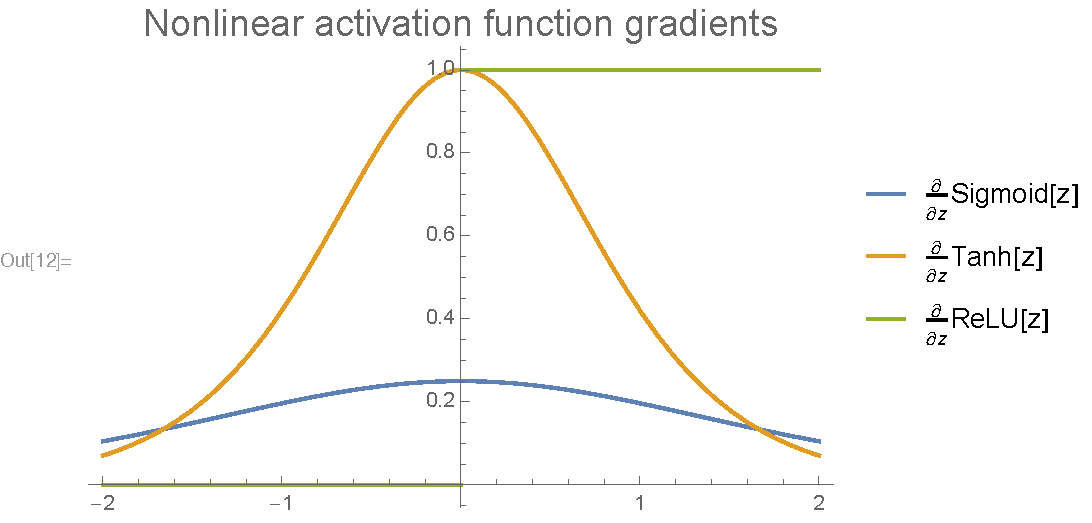
\includegraphics[width=1.00\textwidth]{./figures/nonlinear_activation_gradients.pdf}
  \end{center}
\end{frame}

\end{document}
